\pagestyle{empty} % Limpa o cabeçalho e o rodapé
\onehalfspacing % Espaçamento entre-linhas de 1,5
% \hyphenpenalty=10000 % To prevent hyphenation
\pretolerance=10000 % To avoif overful lines
%\selectlanguage{english}
\setcounter{ex}{0} % counter for exercises
\selectlanguage{brazilian}
%\pagenumbering{arabic} % Uncomment this line if you want renumber pages for each chapter
\renewcommand{\chaptername}{Tutorial}
\chapter{Dados Moleculares - Introdução}\label{tut7}
\rhead{\tiny Instituto de Biociências --USP: BIZ0433 - Inferência Filogenética: Filosofia, Método e Aplicações}
\cfoot{\tiny \cc \ccby \ccsa \href{http://creativecommons.org/licenses/by-sa/4.0/}{Creative Commons Attribution-ShareAlike 4.0 International License}}
%\vspace{5pt}
{\large \sc BIZ0433 - Inferência Filogenética: Filosofia, Método e Aplicações.}\par
%\vspace{10pt}
\par
\minitoc % for table of contents within the chapter
\newpage
\section*{}\addcontentsline{toc}{section}{Objetivo}
\onehalfspacing
\vspace*{5pt}
\begin{center}
\emph{\begin{large}Objetivo\end{large}}\label{tut7:Objetivo}
\vspace{2pt}
\end{center}
%% TEXTO DO RESUMO
O objetivo deste tutorial é apresentar ao aluno algumas ferramentas de manipulação de dados moleculares desde a obtenção de dados no GenBank/NCBI à configurações de matrizes de dados passíveis de serem analisadas em programas de análise filogenética. Ao concluir esse tutorial, o aluno será capaz de reanalisar dados já publicados utilizando TNT. Os arquivos associados a este tutorial estão disponíveis no \href{https://github.com/fplmarques/cladistica/tree/main/tutorials/}{GitHub}. Você baixar todos os tutoriais com o seguinte comando:

\begin{center}
\small \texttt{svn checkout https://github.com/fplmarques/cladistica/trunk/tutorials/}\\
\end{center}


\newpage
\pagestyle{fancy} % Inclui o cabeçalho definido no meta.tex
%\pagenumbering{arabic} % Números das páginas em arábicos
\begin{refsection}
\renewcommand*{\finalnamedelim}{\addspace\&\space}% Usar '&' ao invés de 'e'.

%%%%%%%%%%%%%%%%%%%%%%%%%%%% HERE TEXT STARTS %%%%%%%%%%%%%%%%%%%%%%%%%%%% 
\section{GenBank}\label{tut7:genbank}
\subsection{Formatos de arquivos}\label{tut7:genbank:format}

Antes de entrarmos na parte analítica de dados moleculares é necessário entender alguns formatos de arquivos que contenham dados moleculares. Há vários deles, mas em caráter introdutório iremos apresentar apenas dois. Se você está familiarizado com artigos que usam dados moleculares para inferência filogenética, já deve ter notado que grande parte deles deposita sequências nucleotídicas ou pepitídicas em um repositório chamado GenBank. De fato, todos os periódicos obrigam autores a depositarem esses dados em repositórios como o \textbf{GenBank} e informar aos leitores os números de tombo. Observe a tabela no APPENDIX I de \textcite{dias_et_al_2013}, publicação anexada a este tutorial. As colunas sob o termo ''\textit{GenBank accession number}'' contém os números de tombo das sequências nucleotídicas ou pepitídicas depositadas pelos autores para cada uma das regiões genômicas consideradas nesse estudo (\textit{i.e.}, cyt b, 16S, Rag-1 e 12S). Estes números de tombo permitem que qualquer pessoa verifique e use esses dados.\\

O acesso ao banco de sequências nucleotídicas do GenBank é feito pelo endereço: \url{http://www.ncbi.nlm.nih.gov/nucleotide}. Se você possui um determinado número de tombo, por exemplo FJ685663 -- que de acordo com a tabela apresentada por \textcite{dias_et_al_2013} refere-se ao fragmento de Citocromo B de \textit{Cycloramphus acangatan}--, você poderá obter os dados deste número de tombo simplesmente usando-o na busca disponível nessa página.\\

Por \textit{default}, quando você executa uma busca no GenBank com um único número de tombo, o GenBank retorna o resultado em seu formato mais detalhado. Neste caso em particular isso seria:\\

\scriptsize
\noindent\texttt{Cycloramphus~acangatan~voucher~AF1605~cytochrome~b~(cytb)~gene,~partial~cds;~mitochondrial}

\noindent\texttt{GenBank:~FJ685663.1}

\noindent\texttt{FASTA~Graphics~PopSet}

\noindent\texttt{Go~to:}

\noindent\texttt{LOCUS~~~~~~~FJ685663~~~~~~~~~~~~~~~~~611~bp~~~~DNA~~~~~linear~~~VRT~15-APR-2009}

\noindent\texttt{DEFINITION~~Cycloramphus~acangatan~voucher~AF1605~cytochrome~b~(cytb)~gene,}

\noindent\texttt{~~~~~~~~~~~~partial~cds;~mitochondrial.}

\noindent\texttt{ACCESSION~~~FJ685663}

\noindent\texttt{VERSION~~~~~FJ685663.1~~GI:226510745}

\noindent\texttt{KEYWORDS~~~~.}

\noindent\texttt{SOURCE~~~~~~mitochondrion~Cycloramphus~acangatan}

\noindent\texttt{~~ORGANISM~~Cycloramphus~acangatan}

\noindent\texttt{~~~~~~~~~~~~Eukaryota;~Metazoa;~Chordata;~Craniata;~Vertebrata;~Euteleostomi;}

\noindent\texttt{~~~~~~~~~~~~Amphibia;~Batrachia;~Anura;~Neobatrachia;~Hyloidea;~Cycloramphidae;}

\noindent\texttt{~~~~~~~~~~~~Cycloramphus.}

\noindent\texttt{REFERENCE~~~1~~(bases~1~to~611)}

\noindent\texttt{~~AUTHORS~~~Amaro,R.C.,~Pavan,D.~and~Rodrigues,M.T.}

\noindent\texttt{~~TITLE~~~~~On~the~generic~identity~of~Odontophrynus~moratoi~Jim~\&~Caramaschi,}

\noindent\texttt{~~~~~~~~~~~~1980~(Anura,~Cycloramphidae)}

\noindent\texttt{~~JOURNAL~~~Zootaxa~2071,~61-68~(2009)}

\noindent\texttt{REFERENCE~~~2~~(bases~1~to~611)}

\noindent\texttt{~~AUTHORS~~~Amaro,R.C.,~Pavan,D.~and~Rodrigues,M.T.}

\noindent\texttt{~~TITLE~~~~~Direct~Submission}

\noindent\texttt{~~JOURNAL~~~Submitted~(30-JAN-2009)~Departamento~de~Zoologia,~Instituto~de}

\noindent\texttt{~~~~~~~~~~~~Biociencias,~Universidade~de~Sao~Paulo,~Rua~do~Matao,~ravessa~14,}

\noindent\texttt{~~~~~~~~~~~~101,~Sao~Paulo~05508-090,~Brazil}

\noindent\texttt{FEATURES~~~~~~~~~~~~~Location/Qualifiers}

\noindent\texttt{~~~~~source~~~~~~~~~~1..611}

\noindent\texttt{~~~~~~~~~~~~~~~~~~~~~/organism=''Cycloramphus~acangatan''}

\noindent\texttt{~~~~~~~~~~~~~~~~~~~~~/organelle=''mitochondrion''}

\noindent\texttt{~~~~~~~~~~~~~~~~~~~~~/mol\_type=''genomic~DNA''}

\noindent\texttt{~~~~~~~~~~~~~~~~~~~~~/specimen\_voucher=''AF1605''}

\noindent\texttt{~~~~~~~~~~~~~~~~~~~~~/db\_xref=''taxon:635146''}

\noindent\texttt{~~~~~gene~~~~~~~~~~~~<1..>611}

\noindent\texttt{~~~~~~~~~~~~~~~~~~~~~/gene=''cytb''}

\noindent\texttt{~~~~~CDS~~~~~~~~~~~~~<1..>611}

\noindent\texttt{~~~~~~~~~~~~~~~~~~~~~/gene=''cytb''}

\noindent\texttt{~~~~~~~~~~~~~~~~~~~~~/codon\_start=3}

\noindent\texttt{~~~~~~~~~~~~~~~~~~~~~/transl\_table=2}

\noindent\texttt{~~~~~~~~~~~~~~~~~~~~~/product=''cytochrome~b''}

\noindent\texttt{~~~~~~~~~~~~~~~~~~~~~/protein\_id=''ACO59916.1''}

\noindent\texttt{~~~~~~~~~~~~~~~~~~~~~/db\_xref=''GI:226510746''}

\noindent\texttt{~~~~~~~~~~~~~~~~~~~~~/translation=''LIMQIAPGLFLAMHYTADTSLAFSSIAHICRDVNNGWLLRSLHA}

\noindent\texttt{~~~~~~~~~~~~~~~~~~~~~NGASFFFICIYLHIGRGLYYGSYLFKETWNIGVILLFMTMATAFVGYVLPWGQMSFWG}

\noindent\texttt{~~~~~~~~~~~~~~~~~~~~~ATVITNLLSAAPYIGTDLVQWIWGGFSVDNATLTRFFTFHFILPFIVTGLILLHLIFL}

\noindent\texttt{~~~~~~~~~~~~~~~~~~~~~HETGSSNPTGLNPNPDKVPFHTYFSYKDILGFAIMLSLLASLS''}

\noindent\texttt{ORIGIN~~~~~~}

\noindent\texttt{~~~~~~~~1~gcttaattat~acaaattgca~ccaggactat~tcttagccat~acattacacc~gcggatacct}

\noindent\texttt{~~~~~~~61~cattagcatt~ttcatctatt~gcccatatct~gccgagatgt~aaacaacggg~tgacttcttc}

\noindent\texttt{~~~~~~121~gaagcctcca~cgcaaatggt~gcctcattct~tctttatctg~tatctacctt~catattggcc}

\noindent\texttt{~~~~~~181~gaggattata~ctacggctca~tacttattta~aagaaacatg~aaacattgga~gtgattctcc}

\noindent\texttt{~~~~~~241~tatttataac~catagccaca~gcctttgtcg~gatacgtact~accatgagga~caaatatcat}

\noindent\texttt{~~~~~~301~tctggggggc~cacagtcatc~accaacttat~tatctgcagc~cccctatatt~ggcacagact}

\noindent\texttt{~~~~~~361~tagtgcaatg~aatctgaggc~ggattttcag~tagataacgc~caccctcaca~cgcttcttca}

\noindent\texttt{~~~~~~421~catttcactt~tatcctccca~ttcattgtta~caggattaat~cctcctacac~ctaatctttc}

\noindent\texttt{~~~~~~481~ttcatgaaac~aggatcttca~aaccccacag~gcctaaaccc~taacccagat~aaagtcccat}

\noindent\texttt{~~~~~~541~tccacaccta~cttctcctat~aaagacatcc~taggatttgc~catcatactc~tcccttcttg}

\noindent\texttt{~~~~~~601~cctcactatc~a}
\normalsize

Observe o resultado da busca acima no qual o GenBank lhe fornece uma série de informações sobre essa sequência de nucleotídeos, tais como: autores, região genômica, posicionamento taxonômico do organismo sequenciado, tradução para aminoácidos (para regiões codificantes) e a sequência nucleotídica propriamente dita. Desta forma, este é o formato que contém o maior número de informações sobre a sequência nucleotídica ou peptídica associada ao número de tombo. Minha sugestão é que sempre que possível, obtenha as sequências no Genbank neste formato, pois isso evita ter que revisitar este banco de dados para obter informações adicionais no futuro caso você esteja usando dados disponíveis nesse repositório.\\

Há um outro formato que é muito utilizado na manipulação e análise de sequências nucleotídicas ou pepitídicas: o formato \href{http://pt.wikipedia.org/wiki/Formato\_FASTA}{FASTA}. Na sua forma mais simples, ele contém terminais precedidos de ''>'' e em outra linha a sequência nucleotídica ou pepitídica. Por exemplo:\\

\scriptsize
\noindent\texttt{>sequencia\_1}

\noindent\texttt{ACGTACGTACGT}

\noindent\texttt{>sequencia\_2}

\noindent\texttt{AAGTAAGTAAGT}

\noindent\texttt{>sequencia\_3}

\noindent\texttt{AAATAASTAAAT}

\normalsize

Esse formato é bem simples, útil e frequentemente utilizado para transformar sequências nucleotídicas ou pepitídicas em matrizes de dados. No entanto, este formato permite inserir comentários e outras informações no cabeçalho da sequência. Vejamos por exemplo como o GenBank retornaria a mesma sequência acima (\textit{i.e.}, FJ685663) no formato \href{http://pt.wikipedia.org/wiki/Formato\_FASTA}{FASTA}:\\

\scriptsize
\noindent\texttt{Cycloramphus~acangatan~voucher~AF1605~cytochrome~b~(cytb)~gene,~partial~cds;~mitochondrial}

\noindent\texttt{GenBank:~FJ685663.1}

\noindent\texttt{GenBank~Graphics~PopSet}

\noindent\texttt{>gi|226510745|gb|FJ685663.1|~Cycloramphus~acangatan~voucher~AF1605~cytochrome~b~(cytb) ...}

\noindent\texttt{GCTTAATTATACAAATTGCACCAGGACTATTCTTAGCCATACATTACACCGCGGATACCTCATTAGCATT}

\noindent\texttt{TTCATCTATTGCCCATATCTGCCGAGATGTAAACAACGGGTGACTTCTTCGAAGCCTCCACGCAAATGGT}

\noindent\texttt{GCCTCATTCTTCTTTATCTGTATCTACCTTCATATTGGCCGAGGATTATACTACGGCTCATACTTATTTA}

\noindent\texttt{AAGAAACATGAAACATTGGAGTGATTCTCCTATTTATAACCATAGCCACAGCCTTTGTCGGATACGTACT}

\noindent\texttt{ACCATGAGGACAAATATCATTCTGGGGGGCCACAGTCATCACCAACTTATTATCTGCAGCCCCCTATATT}

\noindent\texttt{GGCACAGACTTAGTGCAATGAATCTGAGGCGGATTTTCAGTAGATAACGCCACCCTCACACGCTTCTTCA}

\noindent\texttt{CATTTCACTTTATCCTCCCATTCATTGTTACAGGATTAATCCTCCTACACCTAATCTTTCTTCATGAAAC}

\noindent\texttt{AGGATCTTCAAACCCCACAGGCCTAAACCCTAACCCAGATAAAGTCCCATTCCACACCTACTTCTCCTAT}

\noindent\texttt{AAAGACATCCTAGGATTTGCCATCATACTCTCCCTTCTTGCCTCACTATCA}

\normalsize

\subsection{Obtendo sequências do GenBank}\label{tut7:genbank:retrieving}

Todos os arquivos de sequências são arquivos texto. Portanto, nada impede que você copie e cole os dados diretamente da página no Genbank no formato que desejar em um editor de texto. Isso porém pode se tornar inviável e extremamente tedioso -- dependendo do número de sequências que você precisa retirar do repositório. O GenBank possui uma ferramenta para retirar sequências nucleotídicas de forma bem eficiente. Essa ferramenta é chamada \textit{Batch Entrez} e pode ser acessada pelo endereço \url{http://www.ncbi.nlm.nih.gov/sites/batchentrez}. A única coisa que você precisa para acessar essa ferramenta é possuir um arquivo texto contendo todos os números de tombo que deseja.\\

	Vejamos o exemplo abaixo. Suponha que você possua um arquivo com o seguinte conteúdo\footnote{ Estes são alguns números de tombo para as sequências de Citocromo B de \textcite{dias_et_al_2013}}:\\
\scriptsize

\noindent\texttt{FJ685663}

\noindent\texttt{FJ685664}

\noindent\texttt{FJ685665}


...


\noindent\texttt{KF214177}

\noindent\texttt{KF214178}

\noindent\texttt{FJ685662}

\normalsize

Basta acessar a página do \textit{Batch Entrez}/Genbank e fazer o \textit{upload} do seu arquivo selecionando a opção \textit{Choose File} (veja Figura \ref{tut7:fig:bacth_entrez}) e em seguida pressionar \textit{Retrieve}.

%%%%%%%%%%%%%%%%%%%%%%%%%%% FIGURA BATCH ENTREZ %%%%%%%%%%%%%%%%%%%%%%%%%%%
%  \vspace{-1em}
  \begin{figure}[H]
    %\ffigbox[\FBwidth]
       \centering
      {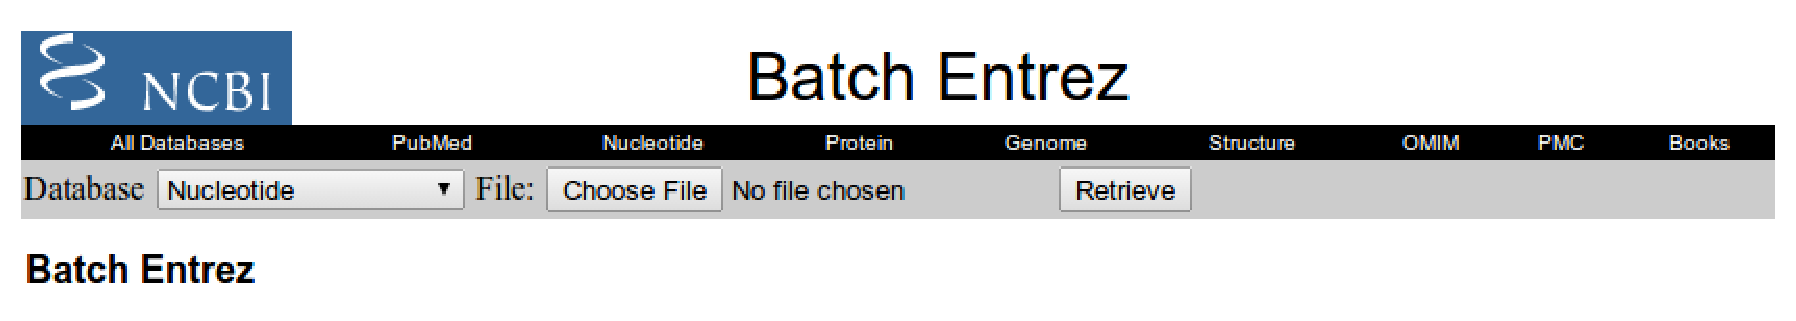
\includegraphics[scale=0.5]{figures/tut7/entrez.eps}}
	{\caption[GenBnank \textit{Batch Entrez}]{Página do \textit{Batch Entrez} do GenBank.}\label{tut7:fig:bacth_entrez}}
  \end{figure}

%%%%%%%%%%%%%%%%%%%%%%%%%%% FIM DA BATCH ENTREZ %%%%%%%%%%%%%%%%%%%%%

Você deverá obter:\\

\scriptsize
\noindent\texttt{Received lines: 40}

\noindent\texttt{Rejected lines: 0}

\noindent\texttt{Removed duplicates: 0}

\noindent\texttt{Passed to Entrez: 40}

\noindent\texttt{Retrieve records for 40 UID(s)}

\normalsize

Neste exemplo em particular, meu arquivo possuía 40 números de tombo e todos eles foram recuperados sem erro.\\
O próximo passo é obter os registros das sequências pressionando ''\texttt{Retrieve records for 40 UID(s)}''. Você deverá obter o resultado ilustrado na Figura \ref{tut7:fig:bacth_entrez_2}.\\

%%%%%%%%%%%%%%%%%%%%%%%%%%% FIGURA BATCH ENTREZ RESULTS %%%%%%%%%%%%%%%%%%%%%%%%%%%
%  \vspace{-1em}
  \begin{figure}[H]
    %\ffigbox[\FBwidth]
       \centering
      {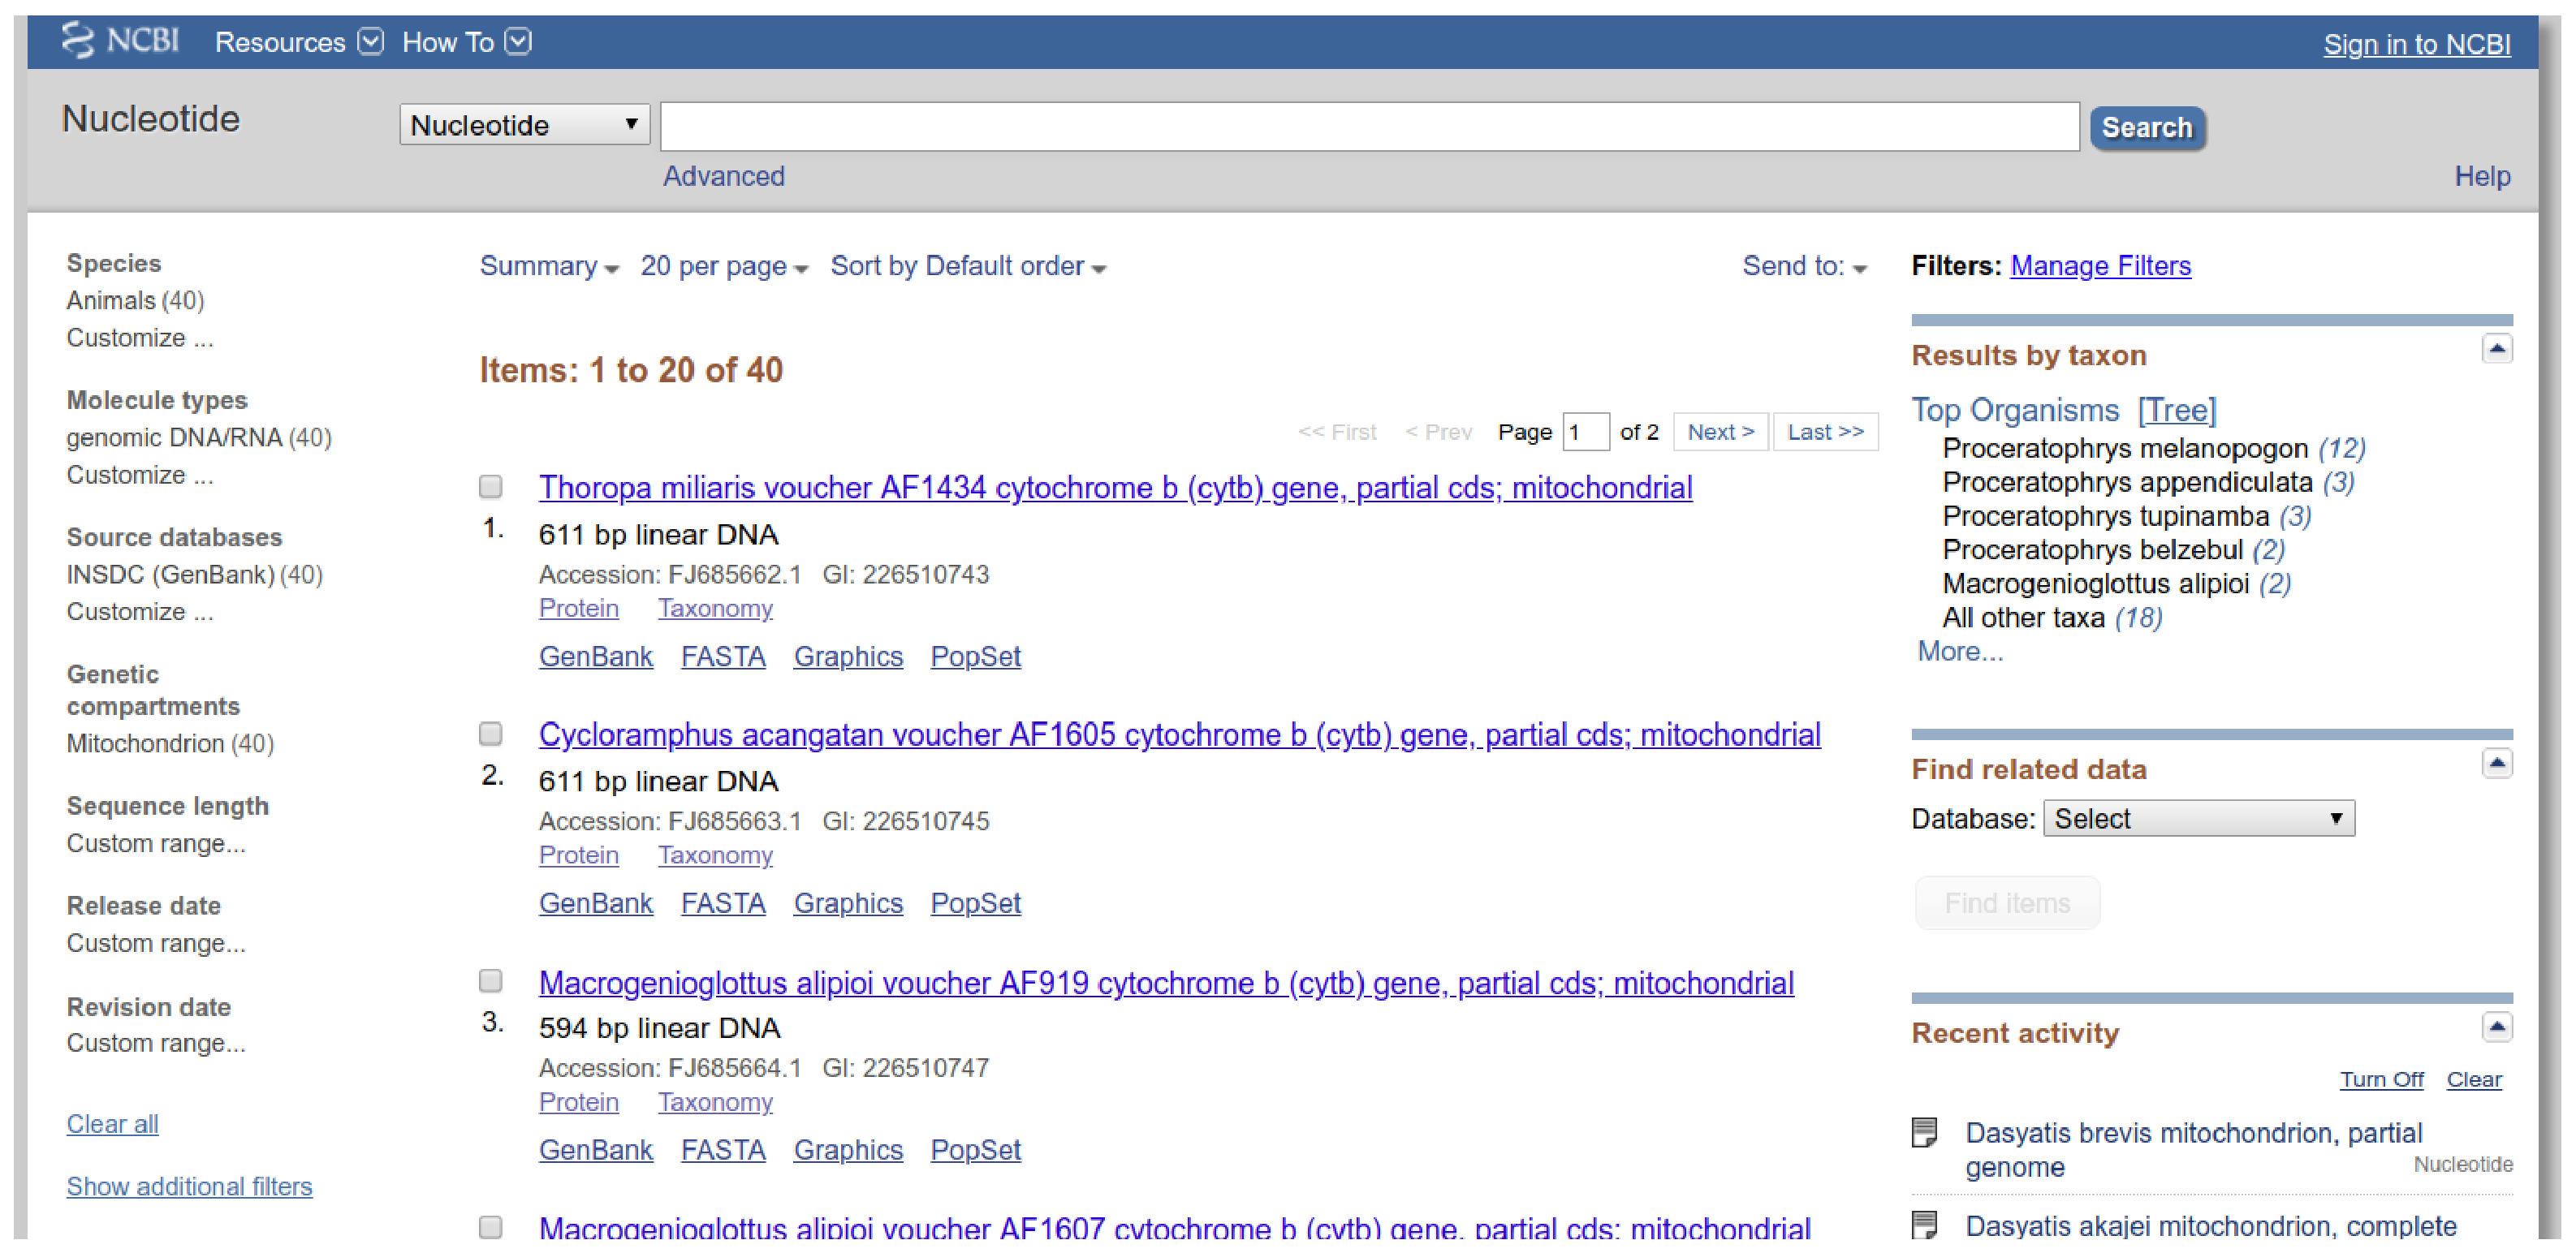
\includegraphics[scale=0.3]{figures/tut7/entrez_2.eps}}
	{\caption[GenBnank \textit{Batch Entrez}: resultado de busca]{Página do \textit{Batch Entrez} do GenBank exibindo resultado de uma busca.}\label{tut7:fig:bacth_entrez_2}}
  \end{figure}

%%%%%%%%%%%%%%%%%%%%%%%%%%% FIM DA BATCH ENTREZ RESULTS %%%%%%%%%%%%%%%%%%%%%

Por \textit{default} o GenBank irá apresentar as sequências solicitadas de forma sumarizada (veja Figura \ref{tut7:fig:bacth_entrez_2}). Isto lhe permite verificar se os números de acesso de fato referem-se às sequências que estava interessado e/ou selecionar parte delas para exame mais detalhado e/ou para baixá-las. Para baixar essas sequências, você precisa definir o formado que deseja utilizar. A definição do formado deve ser selecionada dentre as opções disponíveis nas opções de \textit{Summary} (veja Figura \ref{tut7:fig:display_settings}).

%%%%%%%%%%%%%%%%%%%%%%%%%%% FIGURA BATCH ENTREZ DISPLAY SETTINGS %%%%%%%%%%%%%%%%%%%%%%%%%%%
%  \vspace{-1em}
  \begin{figure}[H]
    %\ffigbox[\FBwidth]
       \centering
      {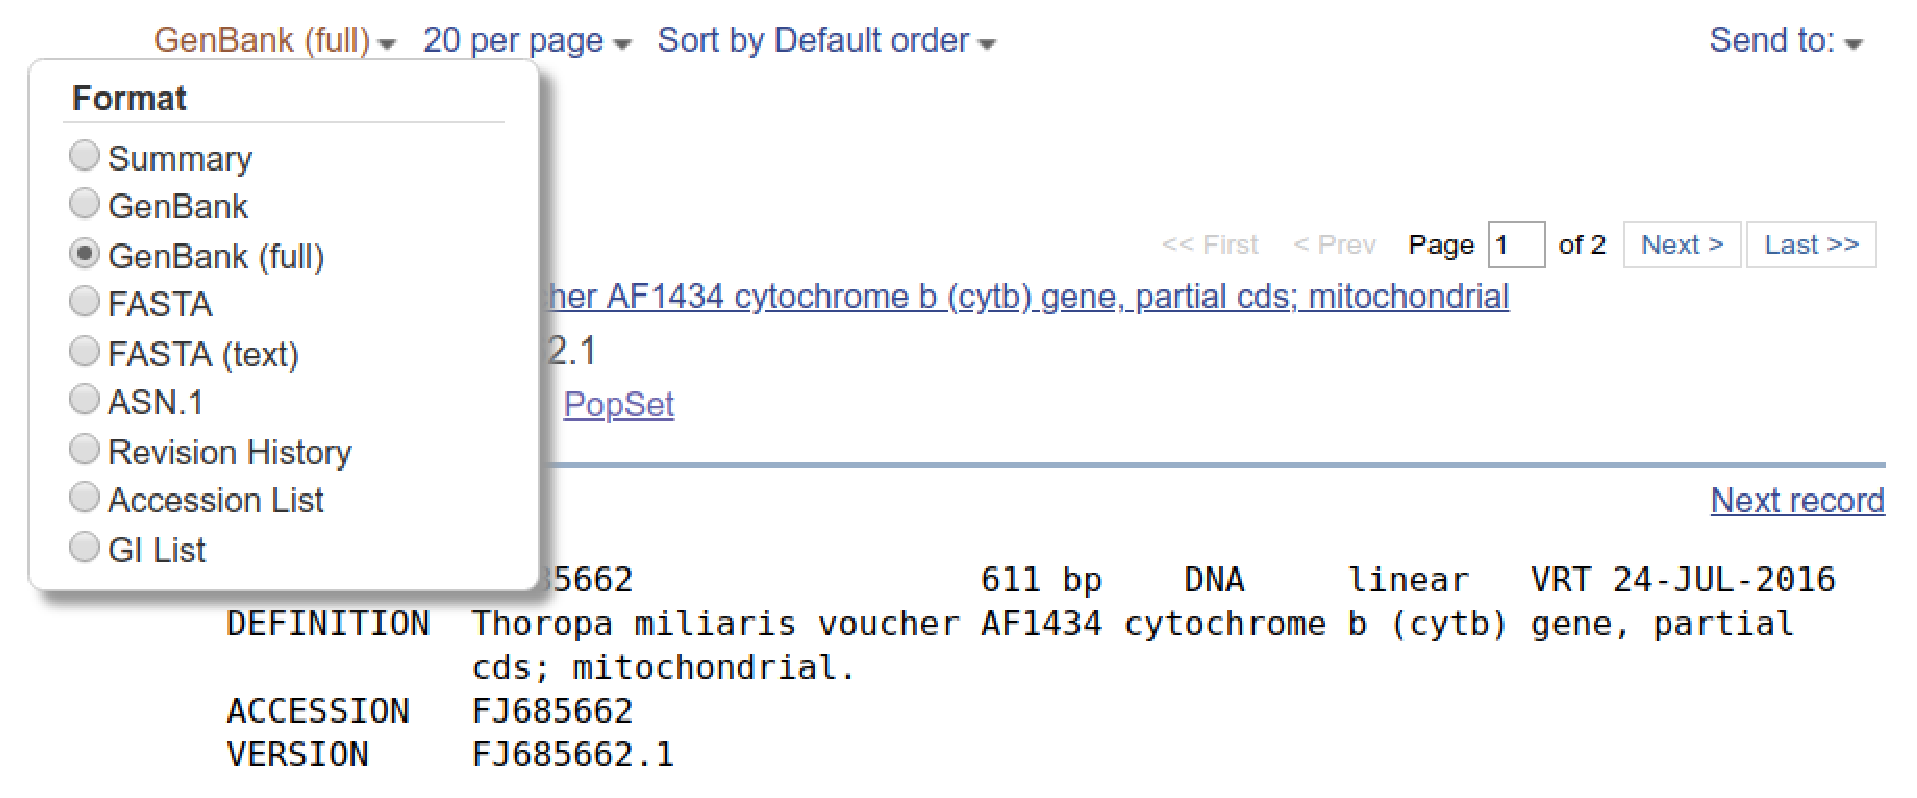
\includegraphics[scale=0.5]{figures/tut7/display_settings.eps}}
	{\caption[GenBnank \textit{Batch Entrez}: seleção de formato de exibição]{Página do \textit{Batch Entrez} do GenBank exibindo as opções para exibição dos resultados de busca.}\label{tut7:fig:display_settings}}
  \end{figure}

%%%%%%%%%%%%%%%%%%%%%%%%%%% FIM DA BATCH ENTREZ DISPLAY SETTINGS %%%%%%%%%%%%%%%%%%%%%

Ao selecionar, por exemplo, o formato \textit{Genbank (full)}, você deverá obter a exibição das sequências no formato referido.\\
No entanto, para baixar as sequências em um determinado formato, não é necessário exibí-las da mesma forma. O \textit{download} de sequências é executado pela seleção das opções em \textit{Send to} (veja Figura \ref{tut7:fig:display_settings}). Ao pressionar \textit{Send to}, você deverá obter uma janela com as opções exibidas na Figura \ref{tut7:fig:send_to_file}.\\

%%%%%%%%%%%%%%%%%%%%%%%%%%% FIGURA BATCH ENTREZ SEND TO %%%%%%%%%%%%%%%%%%%%%%%%%%%
%  \vspace{-1em}
  \begin{figure}[H]
    %\ffigbox[\FBwidth]
       \centering
      {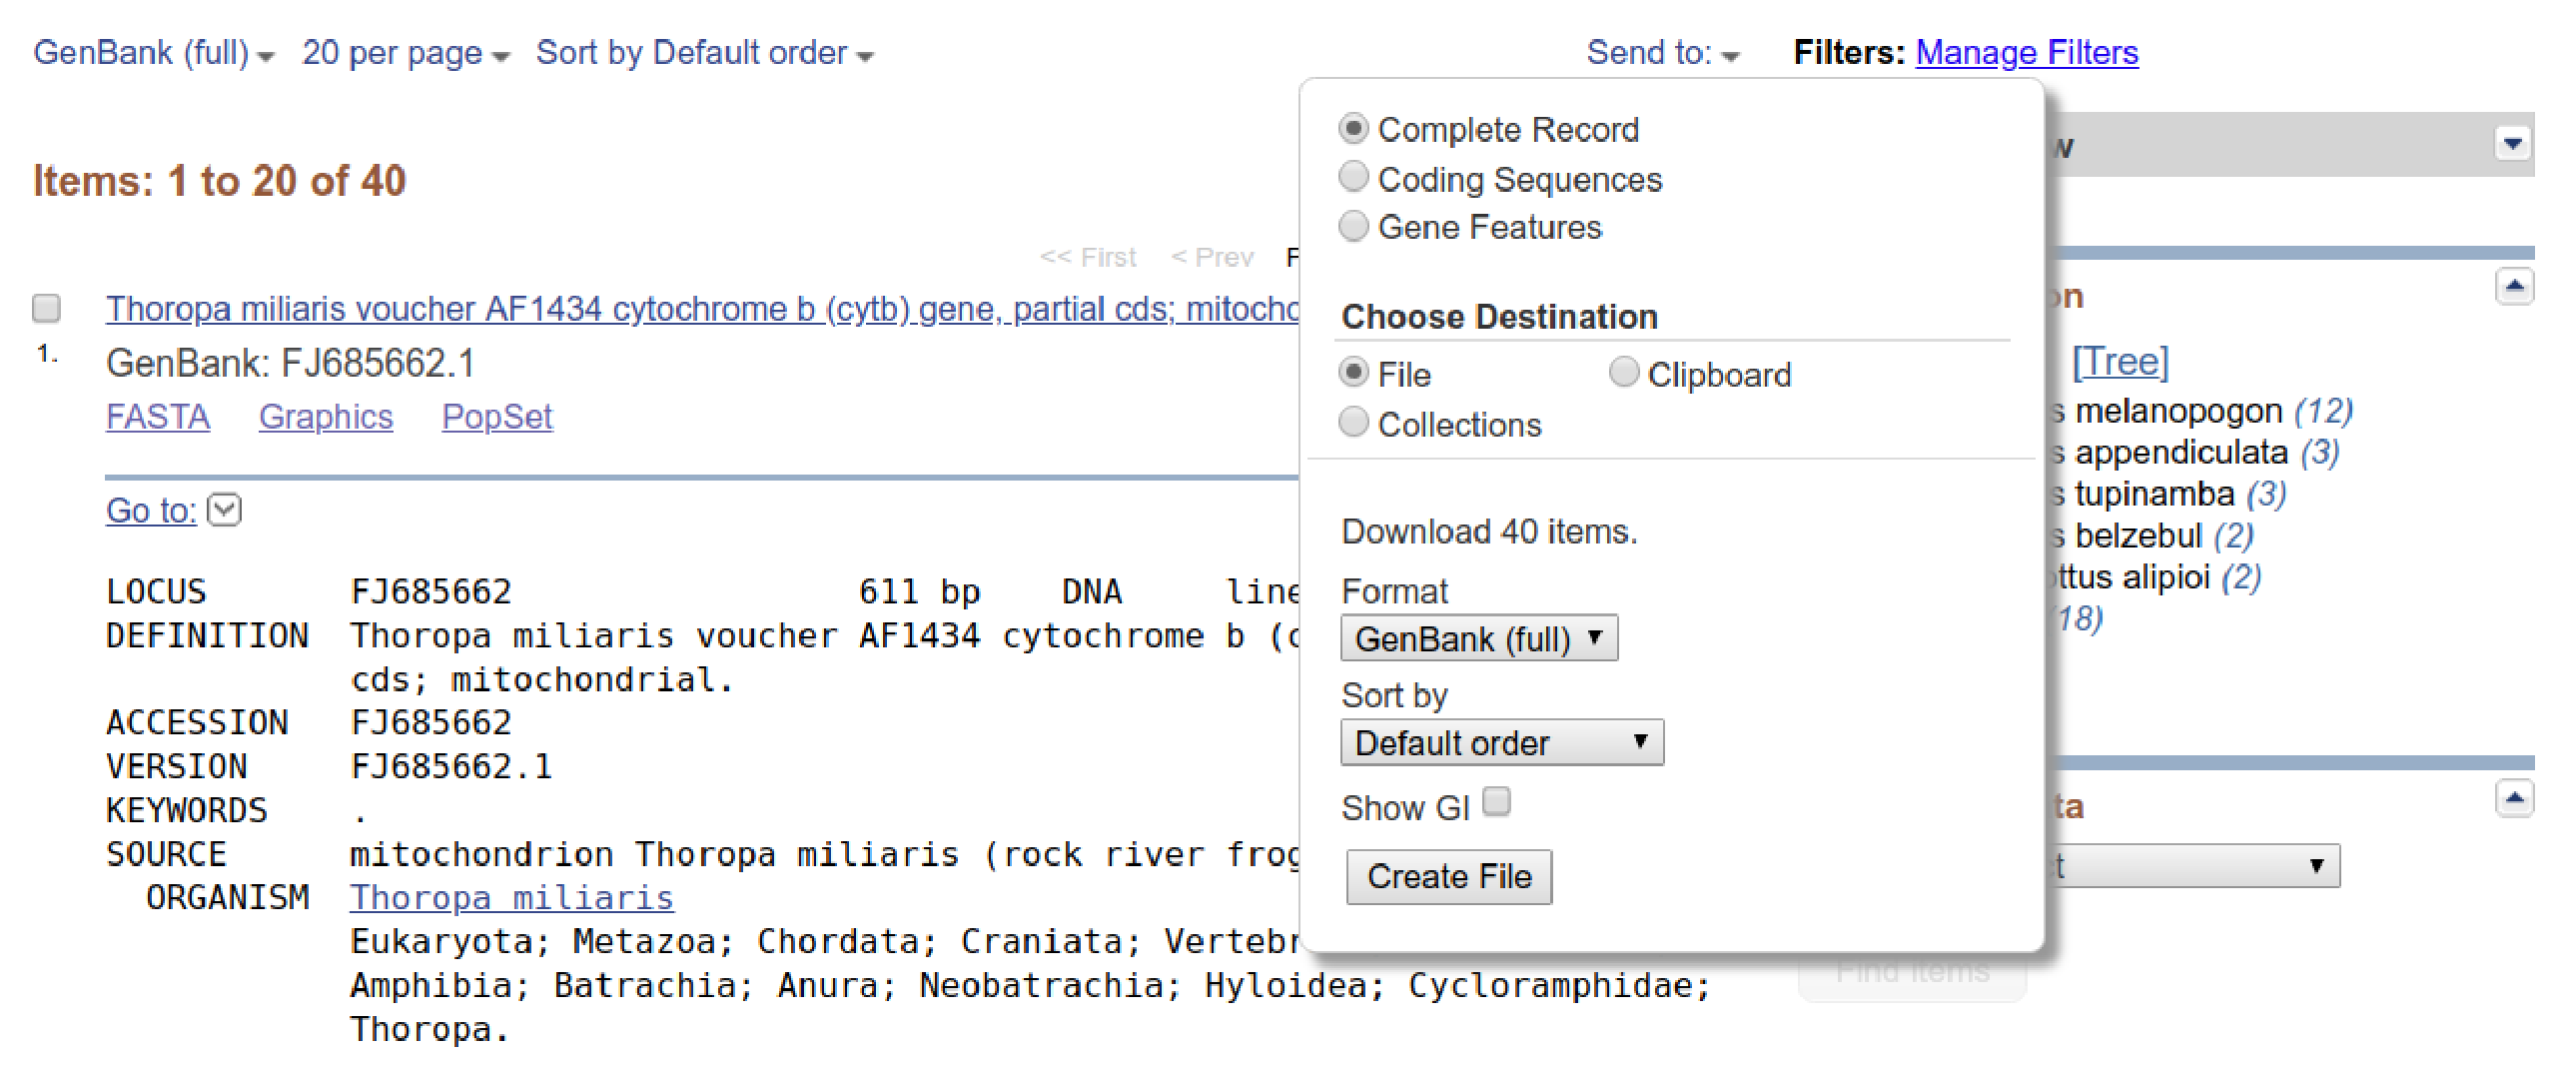
\includegraphics[scale=0.3]{figures/tut7/send_to_file.eps}}
	{\caption[GenBnank \textit{Batch Entrez}: seleção de formato para baixar sequências]{Página do \textit{Batch Entrez} do GenBank exibindo as opções para baixar os resultados de busca.}\label{tut7:fig:send_to_file}}
  \end{figure}

%%%%%%%%%%%%%%%%%%%%%%%%%%% FIM DA BATCH ENTREZ SEND TO %%%%%%%%%%%%%%%%%%%%%

Uma vez selecionadas as opções que deseja nesta janela, basta pressionar \textit{Create File}. O arquivo será salvo com o nome de ''\texttt{sequence.gb}'' no diretório de \textit{default} para \textit{download} de seu sistema. Minha recomendação é que você modifique o nome deste arquivo de forma que seu nome indique seu conteúdo logo após baixar as sequências -- ao fazê-lo, mantenha a extensão ''\texttt{.gb}'' para indicar o formato do arquivo.\\


\stepcounter{ex}
\begin{blackBlock}{\textbf{Exercício 7.\arabic{ex}}}\label{tut7:ex:ex1}

O arquivo ''\texttt{dias\_et\_al\_2013\_accession\_numbers.csv}'' contém todos os números de tombo para as sequências utilizadas por \textcite{dias_et_al_2013} em um arquivo texto no formato CSV (\textit{i.e.}, \textit{Comma Separated Values}). Arquivos neste formato podem ser abertos em programas que manipulam planilhas, tais como EXCEL da Microsoft e OpenOffice Calculator. Este arquivo em particular possui 5 colunas, cada uma referente a uma região genômica utilizada por \textcite{dias_et_al_2013}. Para cada uma destas colunas você deverá

\end{blackBlock}


\begin {myindentpar}{0.3cm}
\begin{enumerate}[\itshape i.]
	\item{Gerar um arquivo texto que contenha apenas os números de tombo referentes a respectiva região genômica. Para cada um dos arquivos, utilize a extensão ``\texttt{.acc}'' -- de \textit{accession} (\textit{e.g}, \texttt{12s.acc}). Esta não é uma extensão particular, somente uma sugestão para que você possa mater seus arquivos organizados.}
 
    \tiny{\textbf{Dica:} Inspecione o arquico em CSV, voce poderia usar a seguinte linha de comando para extrais os números de acesso do cyt-b, que estão na segunda coluna, com a seguinte linha de comando: \texttt{tail -n +2 dias\_et\_al\_2013\_accession\_numbers.csv | cut -d',' -f5 | sed 's/"//g' > 12s.acc}}
    \normalsize
	\item{Utilizar a feramenta do \textit{Batch Entrez} para recuperar os registros referentes a cada um dos arquivos.}

    \tiny{\textbf{Atenção:} Ao fazer o download do GenBank/NCBI o repositório criará um documento chamado \texttt{sequence.gb} que será salvo no diretório de Download de seu sistema.}
    \normalsize
 
	\item{Salvar as sequências de cada região genômica em seus respectivos arquivos no formato \textit{GenBank (full)}. Para cada um dos arquivos, utilize a extensão ``\texttt{.gb}'' -- de \textit{GenBank} (\textit{e.g}, \texttt{12s.gb}).}
\end{enumerate}
\end{myindentpar}

\section{Manipulação de arquivos de sequência}\label{tut7:handling_files}

Nosso objetivo a partir deste momento é extrair as informações dos arquivos gerados pelo GenBank para transformar essas sequências em um arquivo de dados que possa ser analisado por programas de inferência filogenética. No entanto, programas distintos são capazes de ler arquivos em formatos diferentes. No que se segue, manipularemos os arquivos contendo as sequências do Genbank com o objetivo de gerar uma matriz de dados que possa ser analisada em TNT \parencite{GoloboffEtAl_2008}. Os passos apresentados a seguir poderão ser modificados à medida que você se familiarize com as inúmeras ferramentas disponíveis para manipulação de arquivos de sequência. Seja qual for a ferramenta que você venha a escolher no futuro, há dois componentes principais que eu considero importante na preparação de arquivos de sequências para análises filogenéticas. O primeiro deles é o nome dos terminais. O segundo é verificar se as sequências estão alinhadas e no mesmo sentido.

\subsection{Compondo arquivos FASTA}\label{tut7:handling_files:phyloconvert}

Os arquivos no formato \textit{GenBank (full)} possuem um grande número de informações. No entanto, muitas delas não podem ser inseridas em um arquivo que se destine a análise filogenética. Para este último propósito, os nomes dos terminais devem ser curtos e bem definidos e as sequência devem estar alinhadas\footnote{ Alinhamentos serão discutidos com detalhes nos próximos tutoriais.}. O grande número de informações contido nos arquivos no formato \textit{GenBank (full)}, por outro lado, permite que nós possamos extrair o que queremos.\\

A ferramenta que iremos utilizar nesta primeira etapa de manipulação de arquivos de sequência é o \textit{script} chamado  \textit{phyloconvert}. Esse \textit{script} foi concebido primariamente para gerar arquivos no formato FASTA para serem analisados diretamente ou serem subsequentemente transformados em arquivos passíveis de serem analisados em TNT e/ou PAUP \parencite{Swofford_2003,GoloboffEtAl_2008}.\\

O \textit{script} chamado \textit{phyloconvert} faz parte dos aplicativos disponíveis na imagem utilizada no curso, mas caso você não esteja utilizando a imagem, ele está disponível no diretório ''\texttt{tutorial\_7}''. Este \textit{script} requer que BioPython esteja instalado no seu sistema.\\

	A execução do \textit{script} chamado \textit{phyloconvert} é feita do terminal:\\

\shellcmd{phyloconvert}\footnote{Se você quer executar o script que está no diretório você deverá digitar~``\texttt{./phyloconvert}''.}\\

Ao executá-lo você obterá as seguintes opções:\\

\scriptsize

\noindent\texttt{PhyloConvert~0.0.4~-~May~2022~by~Fernando~Marques}\\

\noindent\texttt{\#\#\#\#\#\#\#\#\#\#\#\#\#\#\#\#\#\#\#\#\#\#\#\#\#\#\#\#\#\#\#\#\#\#\#\#\#\#\#\#\#\#\#\#\#\#\#\#\#\#\#\#\#\#\#\#\#\#\#\#\#\#\#\#\#\#\#\#\#\#\#\#\#\#\#\#}

\noindent\texttt{\#~~~~~~~~~~THIS~PROGRAM~CONVERTS~FILES~FOR~PHYLOGENETIC~ANALYSES~~~~~~~~~~~\#}

\noindent\texttt{\#~~~~~~~~~~~~~~~~~~~~~~~~~~~~~~~~~~~~~~~~~~~~~~~~~~~~~~~~~~~~~~~~~~~~~~~~~~\#}

\noindent\texttt{\#~YOUR~OPTIONS~ARE:~~~~~~~~~~~~~~~~~~~~~~~~~~~~~~~~~~~~~~~~~~~~~~~~~~~~~~~~\#}

\noindent\texttt{\#~~~~~~~~~~~~~~~~~~~~~~~~~~~~~~~~~~~~~~~~~~~~~~~~~~~~~~~~~~~~~~~~~~~~~~~~~~\#}

\noindent\texttt{\#~~~1.~For~GenBank~(*.gb)~format~to~FASTA/POY~using~accession~numbers.~~~~~\#}

\noindent\texttt{\#~~~2.~For~GenBank~(*.gb)~format~to~FASTA/POY~using~terminal~names.~~~~~~~~\#}

\noindent\texttt{\#~~~3.~For~GenBank~(*.gb)~format~to~FASTA/POY~using~numbers~and~names.~~~~~\#}

\noindent\texttt{\#~~~4.~For~clean~FASTA~files~to~XREAD~format~(for~TNT).~~~~~~~~~~~~~~~~~~~~\#}

\noindent\texttt{\#~~~5.~For~clean~FASTA~files~to~NEXUS~format~(for~PAUP).~~~~~~~~~~~~~~~~~~~\#}

\noindent\texttt{\#~~~6.~Generate~accession~numbers~list~from~GenBank~(*.gb)~file.~~~~~~~~~~~\#}

\noindent\texttt{\#~~~7.~Generate~taxon~name~list~from~GenBank~(*.gb)~file.~~~~~~~~~~~~~~~~~~\#}

\noindent\texttt{\#~~~8.~Generate~a~file~containing~translation~rules~for~SED.~~~~~~~~~~~~~~~\#}

\noindent\texttt{\#~~~x.~Exit~program.~~~~~~~~~~~~~~~~~~~~~~~~~~~~~~~~~~~~~~~~~~~~~~~~~~~~~~~\#}

\noindent\texttt{\#~~~~~~~~~~~~~~~~~~~~~~~~~~~~~~~~~~~~~~~~~~~~~~~~~~~~~~~~~~~~~~~~~~~~~~~~~~\#}

\noindent\texttt{\#\#\#\#\#\#\#\#\#\#\#\#\#\#\#\#\#\#\#\#\#\#\#\#\#\#\#\#\#\#\#\#\#\#\#\#\#\#\#\#\#\#\#\#\#\#\#\#\#\#\#\#\#\#\#\#\#\#\#\#\#\#\#\#\#\#\#\#\#\#\#\#\#\#\#\#}\\

\noindent\texttt{Select~the~option~desired:}

\normalsize

As três primeiras opções manipulam arquivos no formato \textit{GenBank (full)} transformando-os em arquivos FASTA. A diferença entre estas opções reside na informação que será inserida nos terminais. Por exemplo:\\

\texttt{Select the option desired: 1}\\

\vspace{1.cm}

Resulta em:\\

\scriptsize

\noindent\texttt{>FJ685662}

\noindent\texttt{GCCTAATTACACAAATTATTACAGGACTTTTTTT...}

\noindent\texttt{>FJ685663}

\noindent\texttt{GCTTAATTATACAAATTGCACCAGGACTATTCTT...}

\noindent\texttt{>FJ685664}

\noindent\texttt{GTCACAGGACTCTTCCTTGCAATACACTATACTG...}

\noindent\texttt{...}\\

\normalsize


\texttt{Select the option desired: 2}\\

Resulta em:\\

\scriptsize

\noindent\texttt{>Thoropa\_miliaris}

\noindent\texttt{GCCTAATTACACAAATTATTACAGGACTTTTTTT...}

\noindent\texttt{>Cycloramphus\_acangatan}

\noindent\texttt{GCTTAATTATACAAATTGCACCAGGACTATTCTT...}

\noindent\texttt{>Macrogenioglottus\_alipioi}

\noindent\texttt{GTCACAGGACTCTTCCTTGCAATACACTATACTG...}

\noindent\texttt{...}\\

\normalsize

\texttt{Select the option desired: 3}

Resulta em:\\

\scriptsize

\noindent\texttt{>FJ685662\_Thoropa\_miliaris}

\noindent\texttt{GCCTAATTACACAAATTATTACAGGACTTTTTTT...}

\noindent\texttt{>FJ685663\_Cycloramphus\_acangatan}

\noindent\texttt{GCTTAATTATACAAATTGCACCAGGACTATTCTT...}

\noindent\texttt{>FJ685664\_Macrogenioglottus\_alipioi}

\noindent\texttt{GTCACAGGACTCTTCCTTGCAATACACTATACTG...}

\noindent\texttt{...}\\

\normalsize

A escolha destas opções depende de uma série de fatores. Por exemplo, se sua intenção é concatenar diferentes bases de dados, então você deve escolher a opção que considera apenas o nome dos terminais. Neste caso, assume-se que todas as partições (\textit{i.e.}, distintas regiões genômicas ou diferentes fonte de dados) terão o mesmo nome para cada terminal. No entanto há um problema a considerar. Pode existir no seu banco de dados terminais com o mesmo nome. Neste caso, você terá problemas quando for analisar os dados ou mesmo quando for concatenar as partições -- isso é evidente nesse conjunto de dados. A inserção do número de tombo não permite a concatenação da base de dados, pois cada número é único para determinado táxon e determinada região genômica. No entanto há como contornar esse problema, como veremos adiante. Seja qual for sua opção, pense bem em sua estratégia de análise, pois você poderá encontrar problemas à medida em que executa inúmeras tarefas em seu procedimento analítico.

\stepcounter{ex}
\begin{blackBlock}{\textbf{Exercício 7.\arabic{ex}}}\label{tut7:ex:ex2}

Neste exercício você deverá gerar um arquivo no formato FASTA para cada um dos arquivos que você obteve no Exercício 7.1. Estes arquivos deverão ser criados com a opção \textbf{1} de \textit{phyloconvert}, ou seja, os terminais deverão conter o número de tombo. A razão pela qual não iremos incluir os nomes é porque isso geraria terminais com o mesmo nome e isso seria um problema quando você for concatenar os dados. Por outro lado, a adoção dos números de tombo faria com que cada terminal, em cada partição, fosse considerado como um terminal distinto -- quando, na realidade, você dispõe de 5 regiões genômicas distintas para a grande maioria dos terminais. Portanto esse exercício deverá ser completado por dois procedimentos distintos. No primeiro deles, você irá usar o \textit{phyloconvert} para fazer com que os nomes das sequências recebam o número de tombo do GenBank (opção 1). Na segunda etapa, você deverá substituir os números de tombo pelos nomes dos táxons na primeira coluna do arquivo \texttt{dias\_et\_al\_2013\_accession\_numbers.csv}. Isso será feito com o auxílio do programa \texttt{sed} -- que foi apresentado no Tutorial \ref{tut2}. No diretório \texttt{tutorial\_7} há 5 arquivos de substituição (*\_sub.sed). Após usar o \textit{phyloconvert} você deverá executar o \texttt{sed} utilizando a seguinte linha de comando, por exemplo:\\

\shellcmd{sed -f 12s\_sub.sed 12s.fas > 12s\_renamed.fas}
\end{blackBlock}

A opção \texttt{-f} diz ao \texttt{sed} que as instruções de substituição estão no arquivo \texttt{12s\_sub.fas} que serão aplicadas ao arquivo \texttt{12s.fas} e o resultado será redirecionado (\texttt{>}) para o arquivo \texttt{12s\_renamed.fas}.

\subsection{Verificação e edição FASTA em AliView}\label{tut7:handling_files:AliView}

Uma vez editado os nomes dos terminais é necessário verificar as sequências nucleotídicas e, via de regra, editar o arquivo. Para isso usaremos o aplicativo chamado \href{https://ormbunkar.se/aliview/}{AliView} \parencite{larson_2014}. AliView é uma aplicativo muito útil e intuitivo de usar. Há outras ferramentas disponíveis para esse propósito, tais como \href{http://pbil.univ-lyon1.fr/software/seaview3.html#:~:text=SeaView%20is%20a%20graphical%20multiple,to%20locally%20improve%20the%20alignment.}{SeaView} e \href{https://www.geneious.com/}{Geneious} -- entre outros, caso ele não atenda suas necessidades. Para os propósitos de nosso curso, ele será suficiente.

O AliView é iniciado em um terminal. Abra um terminal e execute o comando \texttt{aliview}. Após a execução, você deverá obter a janela do programa tal qual na Figura \ref{tut7:fig:AliView}.


%%%%%%%%%%%%%%%%%%%%%%%%%%% FIGURA AliView %%%%%%%%%%%%%%%%%%%%%%%%%%%
%  \vspace{-1em}
  \begin{figure}[H]
    %\ffigbox[\FBwidth]
       \centering
      {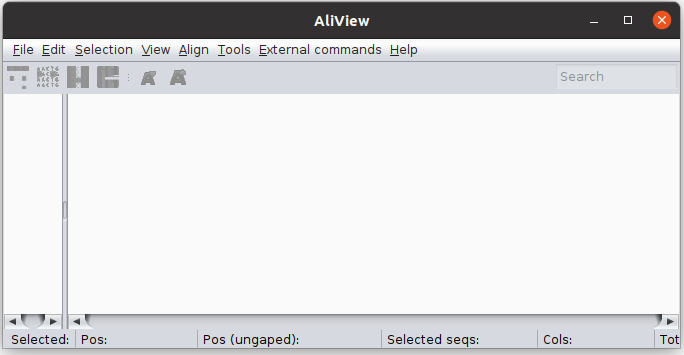
\includegraphics[scale=0.5]{figures/tut7/aliview_01.png}}
	{\caption[AliView: janela inicial]{Janela inicial do AliView.}\label{tut7:fig:AliView}}
  \end{figure}

%%%%%%%%%%%%%%%%%%%%%%%%%%% FIM DA FIGURA AliView %%%%%%%%%%%%%%%%%%%%%

Para demonstrar alguns atributos de AliView, eu irei apresentar uma série comandos no programa utilizando o arquivo \texttt{exemplo\_aliwiew\_cyt-b.fas} que encontra-se disponível no diretório \texttt{tutorial\_07}. Esse arquivo foi gerado a partir das sequências de Citocromo B de \textcite{dias_et_al_2013} após eu ter criado um arquivo FASTA (usando a opção 1) utilizando o \textit{script} \texttt{phyloconvert}, como vocês fizeram no Exercício 7.1.\\

No AliView, vá em \textbf{File > Open} File e abra o arquivo \texttt{exemplo\_aliwiew\_cyt-b.fas} que está no diretório \texttt{tutorial\_07}. Uma vez aberto, corra a barra de rolagem horizontal até o final das sequências nucleotídicas como ilustrado na Figura \ref{tut7:fig:AliView_2}.

%%%%%%%%%%%%%%%%%%%%%%%%%%% FIGURA AliView 2 %%%%%%%%%%%%%%%%%%%%%%%%%%%
%  \vspace{-1em}
  \begin{figure}[H]
    %\ffigbox[\FBwidth]
       \centering
      {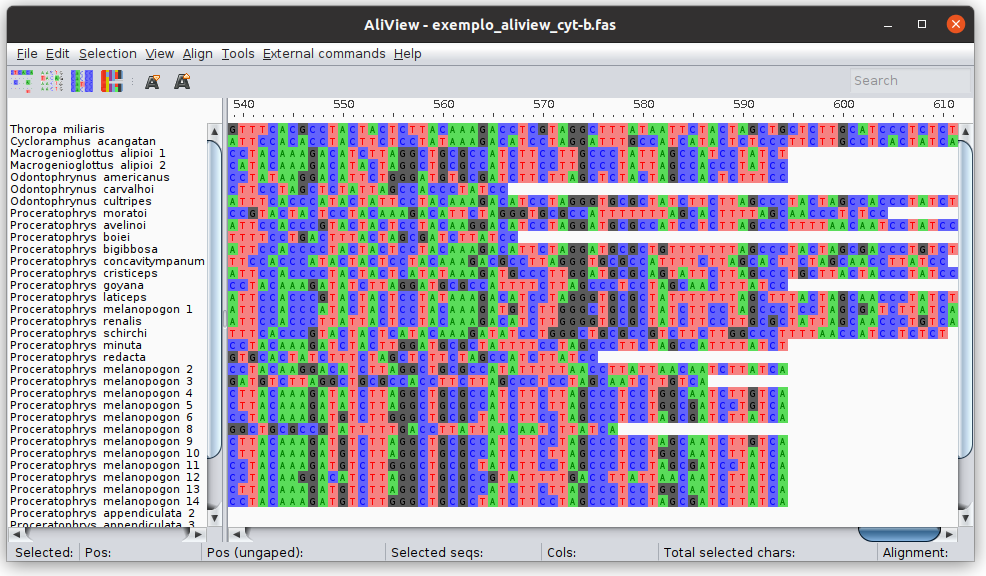
\includegraphics[scale=0.4]{figures/tut7/aliview_02.png}}
	{\caption[AliView]{Arquivo \texttt{exemplo\_aliwiew\_cyt-b.fas} aberto no AliView.}\label{tut7:fig:AliView_2}}
  \end{figure}

%%%%%%%%%%%%%%%%%%%%%%%%%%% FIM DA FIGURA AliView 2 %%%%%%%%%%%%%%%%%%%%%


Você deverá observar que no arquivo \texttt{exemplo\_aliview\_cyt-b.fas} as sequências nucleotídicas diferem de tamanho (Figura \ref{tut7:fig:AliView_2}). Estas diferenças se dão por sequenciamento diferencial das amostras. Adicionalmente, o Citocromo B é um gene codificante, onde raramente ocorrem inserções e deleções e quando ocorrem tendem a atuar sobre códon -- portanto três nucleotídios. Para que possamos proceder com análises filogenéticas desses dados é necessário alinhar essas sequências.  Alinhamento é o processo pelo qual sequências de tamanhos diferentes são igualadas quanto ao tamanho com a inserção de \textit{gaps} (``-''). Nós iremos discutir detalhadamente algoritmos de alinhamento e a relação entre alinhamento e hipóteses filogenéticas no próximo tutoria. No momento, por se tratar de uma região codificadora, a expectativa é que os \textit{gaps} sejam inseridos no começo e no final de cada sequência.\\


O alinhamento de sequências em AliView requer inicialmente que todas as sequências sejam selecionadas. Para fazer isso clique em \textbf{Selection > Select all}. Uma vez selecionadas, clique em \textbf{Align > Realign everything} e clique em OK para iniciar o alinhamento. Na configuração padrão de AliView, o programa de alinhamento é o \href{https://www.ebi.ac.uk/Tools/msa/muscle/}{Muscle} -- que será discutido no próximo tutorial. Quando o processo de alinhamento terminar -- indicado pela mensagem ``\texttt{Done}'', feche a janela \texttt{Align with Muscle}. O resultado final deverá ser semelhante ao que é apresentado na Figura \ref{tut7:fig:AliView_aligned}.


%%%%%%%%%%%%%%%%%%%%%%%%%%% FIGURA AliView EXAMPLE %%%%%%%%%%%%%%%%%%%%%%%%%%%
%  \vspace{-1em}
  \begin{figure}[h!]
    %\ffigbox[\FBwidth]
       \centering
      {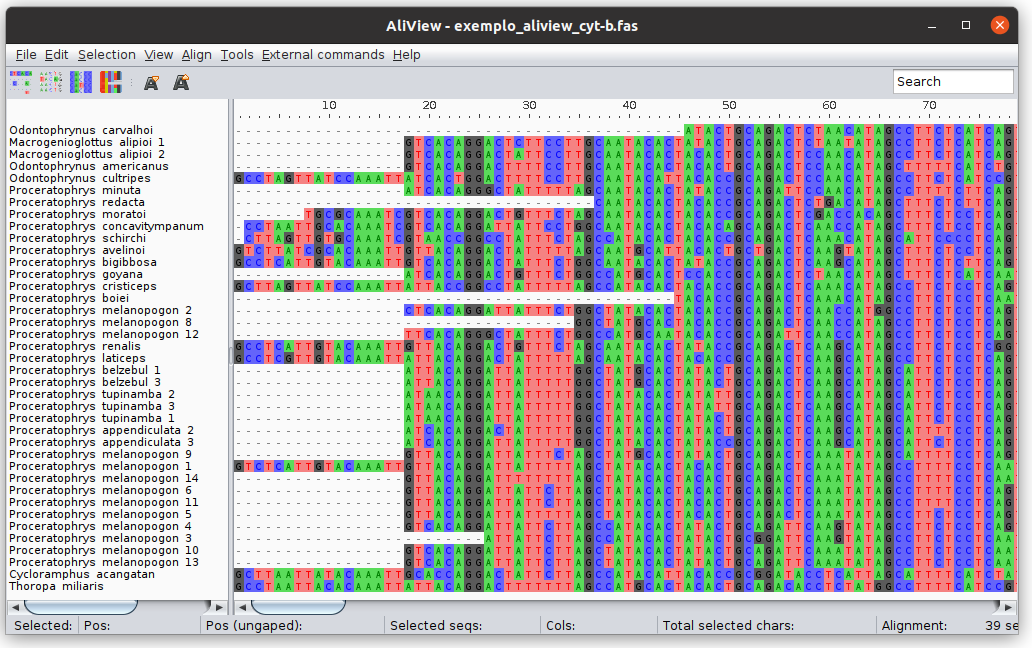
\includegraphics[scale=0.4]{figures/tut7/aliview_03.png}}
	{\caption[AliView: alinhamento]{Alinhamento via Muscle em AliView das sequências em \texttt{exemplo\_aliview\_cyt-b.fas}.}\label{tut7:fig:AliView_aligned}}
  \end{figure}

%%%%%%%%%%%%%%%%%%%%%%%%%%% FIM DA FIGURA AliView EXAMPLE %%%%%%%%%%%%%%%%%%%%%

Observe que após esse procedimento todas as sequências possuem o mesmo comprimento (612 pares de base [bp]). O Muscle inseriu a maioria dos \textit{gaps} na porção inicial das sequências, chamados \textit{leading gaps}, nenhum \textit{gap} no meio das sequências, e algumas sequências com \textit{gaps} no final, estes chamados de \textit{trailling gaps}. Os \textit{gaps} iniciais e finais resultam do processo de sequenciamento diferencial para cada terminal. Se as sequências são mantidas como estão, estes \textit{gaps} podem ser considerados como um quinto estado de caráter (\textit{i.e.}, A, C, G, T e -) quando não deveriam. Desta forma, é necessário editar as regiões iniciais destas sequências. Isso pode ser feito de duas formas. Uma delas é removendo as regiões iniciais das sequências, a outra forma é substituindo os \textit{gaps} por ``\texttt{N}s''. Considere que a substituição de \textit{leading} e \textit{trailling gaps} por ``\texttt{N}'' insere ambiguidade nos dados, pois ``\texttt{N}'' é considerado como ``\texttt{?}'' durante análises filogenéticas. Por outro lado, a remoção destas regiões pode resultar na perda de dados que pode ser importante para resolver a topologia. Por exemplo, há 7 sequências em que há \~300 pares de base faltantes no final. Isso levou a inserção de muitos \textit{gaps}. Se você optar pela exclusão desta região, você perde a metade dos seus dados aproximadamente. A decisão entre remover ou substituir é arbitrária.\\

Neste exemplo iremos fazer os dois procedimentos. O primeiro deles é remover os 17 pares de base da região inicial do alinhamento. Para remover esta região no AliView basta você selecionar esta região com o mouse e pressionar \texttt{Ctrl+Del}. Você deverá obter o que é ilustrado na Figura\ref{tut7:fig:AliView_trimmed}.


%%%%%%%%%%%%%%%%%%%%%%%%%%% FIGURA AliView EXAMPLE %%%%%%%%%%%%%%%%%%%%%%%%%%%
%  \vspace{-1em}
  \begin{figure}[H]
    %\ffigbox[\FBwidth]
       \centering
      {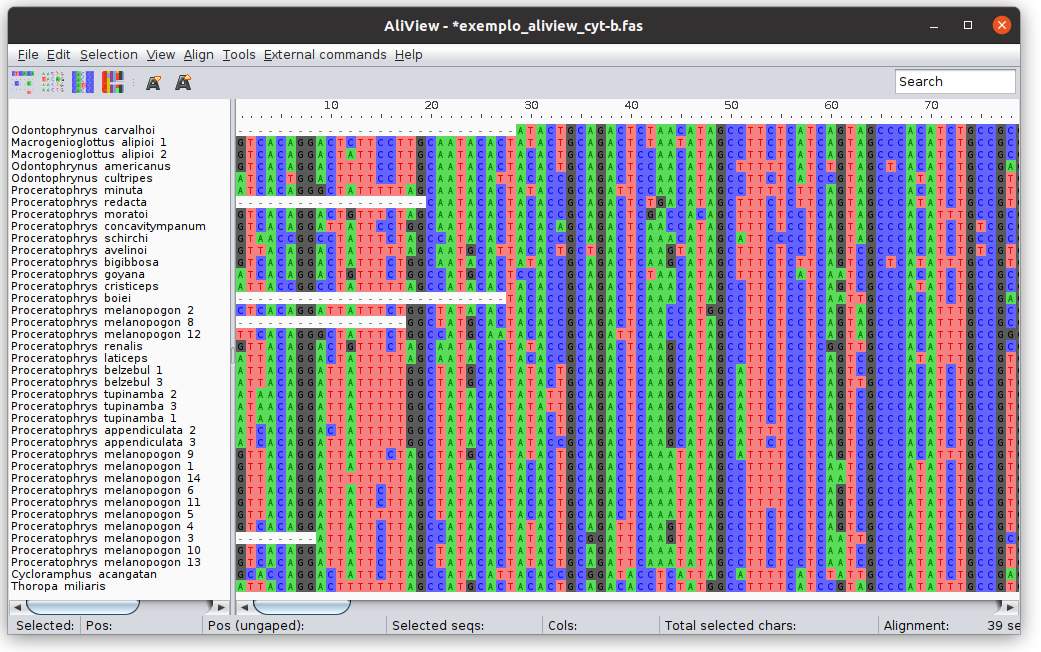
\includegraphics[scale=0.4]{figures/tut7/aliview_04.png}}
	{\caption[AliView: remoção da região inicial]{Arquivo \texttt{exemplo\_aliview\_cyt-b.fas} com a remoção dos primeiros 17 pares de base.}\label{tut7:fig:AliView_trimmed}}
  \end{figure}

%%%%%%%%%%%%%%%%%%%%%%%%%%% FIM DA FIGURA AliView EXAMPLE %%%%%%%%%%%%%%%%%%%%%

O segundo passo será transformar os \textit{gaps} iniciais e finais em ``\texttt{N}s''. Isso pode ser feito de duas formas. A primeira delas é manualmente, mas isso pode ser indesejável quando o número de sequências é relativamente grande, a outra é usando um \textit{script} que faz isso por você. Vamos usar as duas estratégias. Para fazer isso manualmente na região inicial, basta selecionar a região de \textit{gaps} de uma determinada sequência e pressionar a tecla ``\texttt{n}''. Você deverá obter o que está ilustrado na Figura \ref{tut7:fig:AliView_init}. A segunda forma é utilizar o \textit{script} \texttt{subedgesgaps.py} para executar a mesma tarefa, mas agora na região final das sequências nucleotídicas. Para isso, eu vou salvar este alinhamento parcialmente editado em \textbf{File > Save as Fasta} sob o nome de \texttt{exemplo\_aliview\_cyt-b\_aln\_trim.fas} e vou fechar o AliView.


%%%%%%%%%%%%%%%%%%%%%%%%%%% FIGURA AliView EXAMPLE %%%%%%%%%%%%%%%%%%%%%%%%%%%
%  \vspace{-1em}
  \begin{figure}[H]
    %\ffigbox[\FBwidth]
       \centering
      {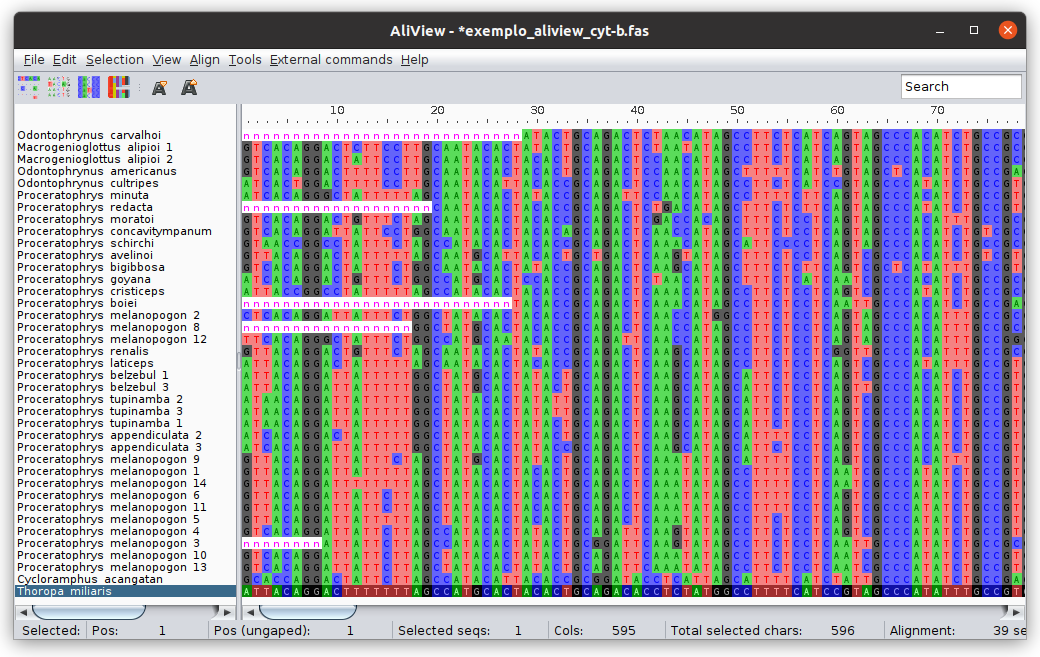
\includegraphics[scale=0.4]{figures/tut7/aliview_05.png}}
	{\caption[AliView: edição da região inicial]{Inserção manual de ``\texttt{N}s'' na região inicial do alinhamento.}\label{tut7:fig:AliView_init}}
  \end{figure}

%%%%%%%%%%%%%%%%%%%%%%%%%%% FIM DA FIGURA AliView EXAMPLE %%%%%%%%%%%%%%%%%%%%%
%%%%%%%%%%%%%%%%%%%%%%%%%%% FIGURA AliView EXAMPLE %%%%%%%%%%%%%%%%%%%%%%%%%%%
%  \vspace{-1em}
  \begin{figure}[H]
    %\ffigbox[\FBwidth]
       \centering
      {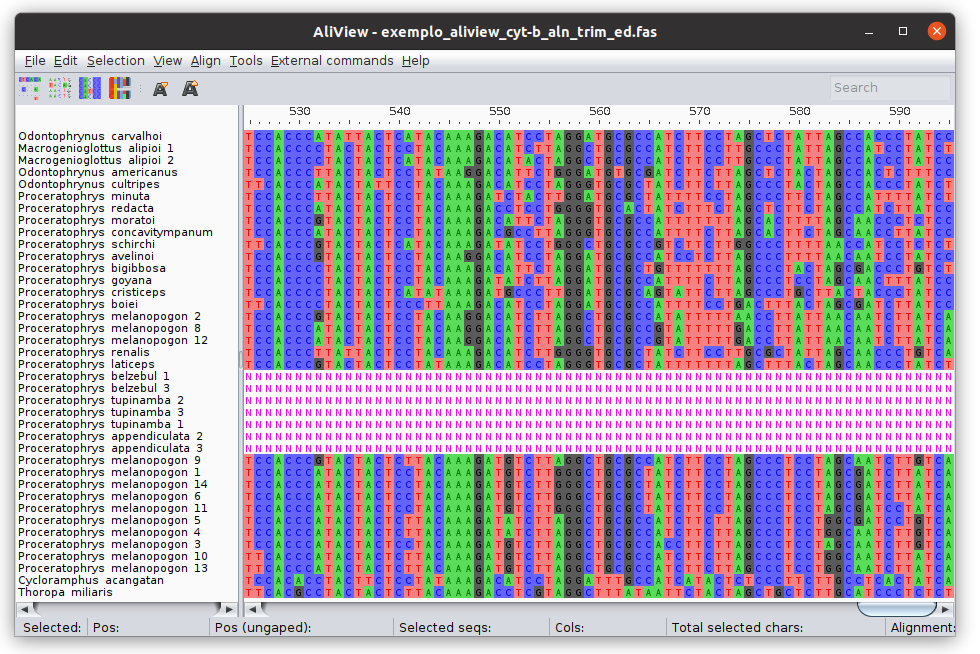
\includegraphics[scale=0.4]{figures/tut7/aliview_06.png}}
	{\caption[AliView: edição da região final]{Inserção de ``\texttt{N}s'' na região final do alinhamento utilizando o \textit{script} \texttt{subedgesgaps.py}.}\label{tut7:fig:AliView_end}}
  \end{figure}

%%%%%%%%%%%%%%%%%%%%%%%%%%% FIM DA FIGURA AliView EXAMPLE %%%%%%%%%%%%%%%%%%%%%

Agora vamos editar a parte final deste alinhamento utilizando o \textit{script} \texttt{subedgesgaps.py}. Essa operação é relativamente simples. Em um terminal execute o seguinte comando:

\shellcmd{python3 subedgesgaps.pl -i exemplo\_aliview\_cyt-b\_aln\_trim.fas > exemplo\_aliview\_cyt-b\_aln\_trim\_ed.fas}\\


Se abrirmos o arquivo \texttt{exemplo\_aliview\_cyt-b\_aln\_trim\_ed.fas} no AliView e observarmos o final do alinhamento iremos ver que todos aqueles \textit{gaps} terminais foram preenchidos com ``\texttt{N}s'' como ilustrado na Figura \ref{tut7:fig:AliView_end}. Essa estratégia poderia ter sido adotada logo no início,  após a deleção dos primeiros 17 pares de base. A operação anterior foi simplesmente para demonstrar que o AliView permite a edição das sequências manualmente.


Recomendo que em cada etapa de edição parcial você salve o arquivo editado sob outro nome. Geralmente eu uso a notação ``\texttt{\_aln}'' para arquivos editados, ``\texttt{\_trim}'' para arquivos em que eu removi as regiões iniciais e\/ou finais (de \textit{trimmed}) e ``\texttt{\_ed}'' quando eu implemento edições. Isso possibilita que você volte a alguma etapa anterior caso detecte algum erro. Seu objetivo é chegar a uma edição final no qual o arquivo está no formato compatível com o programa de inferência filogenética que você deseja utilizar, incluindo como as regiões de inserção e deleção devam ser tratadas. Uma última ponderação sobre o exemplo acima; em alguns casos, o alinhamento apresentará \textit{gaps} internos. Para genes ribossomais, estes devem ser tratados como quinto estado de caráter. Em regiões codificantes, a existência desses \textit{gaps} não é usual e deve ser acompanhada de \textit{triplets} -- três \textit{gaps} via de regra.

\vspace{0.5cm}

\stepcounter{ex}
\begin{blackBlock}{\textbf{Exercício 7.\arabic{ex}}}\label{tut7:ex:ex3}

Para que você se familiarize com o AliView, você deverá editar e salvar as edições de todos os arquivos que você gerou no Exercício 7.1.

\end{blackBlock}


\section{Configuração de matrizes de dados moleculares}\label{tut7:matrices}

Transformar um arquivo FASTA em um arquivo passível de análises filogenéticas é relativamente simples -- embora em alguns casos isso seja desnecessário como veremos ao longo desses tutoriais. Como vocês estão familiarizados com o formato de arquivos de entrada para TNT (veja Seção \ref{tut4:input} do Tutorial \ref{tut4}), iremos explorar como tramsformar um arquivo FASTA em formato \texttt{xread}.\\

	Considere as seguintes sequências em formato FASTA:\\

\scriptsize

\noindent\texttt{>taxon\_1}

\noindent\texttt{GCCTAATTACACAAATTATT}

\noindent\texttt{>taxon\_2}

\noindent\texttt{GCTTAATTATACAAATTGCA}

\noindent\texttt{>taxon\_3}

\noindent\texttt{GTCACAGGACTCTTCCTTGC}

\noindent\texttt{>taxon\_4}

\noindent\texttt{GTCACAGGACTCATACACTA}


\normalsize

\vspace{0.5cm}

Neste exemplo temos 4 terminais com sequências de 20 pares de base. A edição deste arquivo para que seja passível de análise filogenética em TNT é simples e pode ser feita manualmente. Veja como seria:\\


\scriptsize

\noindent\texttt{nstates dna;}

\noindent\texttt{xread}

\noindent\texttt{20 4}


\noindent\texttt{taxon\_1~~~~~GCCTAATTACACAAATTATT}


\noindent\texttt{taxon\_2~~~~~GCTTAATTATACAAATTGCA}


\noindent\texttt{taxon\_3~~~~~GTCACAGGACTCTTCCTTGC}


\noindent\texttt{taxon\_4~~~~~GTCACAGGACTCATACACTA;}

\noindent\texttt{proc/;}


\normalsize

ou ainda:\\

\scriptsize

\noindent\texttt{xread}

\noindent\texttt{20 4}


\noindent\texttt{taxon\_1~~~~~21130033010100033033}


\noindent\texttt{taxon\_2~~~~~21330033030100033210}


\noindent\texttt{taxon\_3~~~~~23101022013133113321}


\noindent\texttt{taxon\_4~~~~~23101022013103010130;}

\noindent\texttt{proc/;}\\


\normalsize

No primeiro caso, as sequências estão inseridas como vieram do arquivo FASTA e isso requer que a primeira linha do arquivo contenha ''\texttt{nstates dna;}''. No segundo caso, o arquivo é idêntico aos que vocês já viram anteriormente. Neste caso, as bases \texttt{A, C, G} e \texttt{T} foram substituídas por \texttt{0, 1, 2} e \texttt{3}, respectivamente. Para arquivos simples como esse, a edição manual é possível, mas pode se tornar inviável à medida em que o número de terminais e/ou de pares de base aumentam. Neste caso, o melhor a fazer é usar \textit{scripts} ou aplicativos concebidos para esse propósito.\\

Como vocês viram na seção \ref{tut7:handling_files:phyloconvert}, o \textit{script} \textit{phyloconvert} possui duas opções que possibilitam a configuração de arquivos para TNT e PAUP a partir de arquivos FASTA (opções 4 e 5, veja acima). Acredito que não terá dificuldades em usar \textit{phyloconvert} para transformar arquivos no formato FASTA em arquivos para TNT e PAUP. Portanto, vamos explorar outra ferramenta.\\

	\subsection{SequenceMatrix}\label{tut7:matrices:sequencematrix}

    \href{https://code.google.com/p/sequencematrix/}{SequenceMatrix}
	\parencite{Vaidya_et_all_2010} é um aplicativo relativamente simples, mas muito útil para transformar arquivos FASTA em outros formatos. O aplicativo também permite concatenar bancos de dados distintos de forma muito amigável. \href{https://code.google.com/p/sequencematrix/}{SequenceMatrix} tem uma série de funções que não serão exploradas em detalhe neste tutorial, consulte a página do aplicativo e o trabalho de \textcite{Vaidya_et_all_2010} para maiores informações. Vejamos como ele funciona considerando as três partições ilustradas na Figura \ref{tut7:fig:partitions}.

%%%%%%%%%%%%%%%%%%%%%%%%%%% FIGURA AliView EXAMPLE %%%%%%%%%%%%%%%%%%%%%%%%%%%
%  \vspace{-1em}
  \begin{figure}[H]
    %\ffigbox[\FBwidth]
       \centering
      {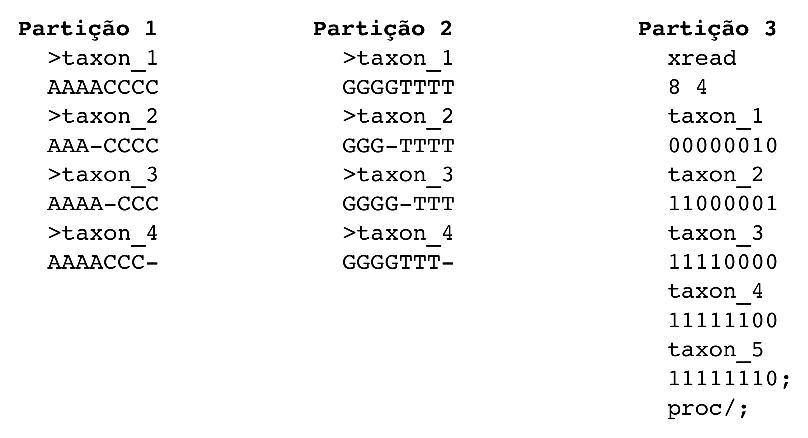
\includegraphics[scale=1.0]{figures/tut7/partitions.eps}}
	{\caption[Três exemplos de partições de dados]{Partições de dados utilizadas no exemplo de SequenceMatrix. As duas primeiras partições estão em formato FASTA. A terceira partição é uma arquivo para dados morfológicos no formato \texttt{xread} de TNT. Observe que a terceira partição contém um terminal a mais que as demais.}\label{tut7:fig:partitions}}
  \end{figure}

%%%%%%%%%%%%%%%%%%%%%%%%%%% FIM DA FIGURA AliView EXAMPLE %%%%%%%%%%%%%%%%%%%%%

A execução do \texttt{SequenceMatrix} é feita do terminal da sequinte forma:\\

\shellcmd{sequencematrix}\\

Ao executá-lo você deverá obter a sequinte janela:\\

%%%%%%%%%%%%%%%%%%%%%%%%%%% FIGURA SEQUENCEMATRIX 1 %%%%%%%%%%%%%%%%%%%%%%%%%%%
%  \vspace{-1em}
  \begin{figure}[H]
    %\ffigbox[\FBwidth]
       \centering
      {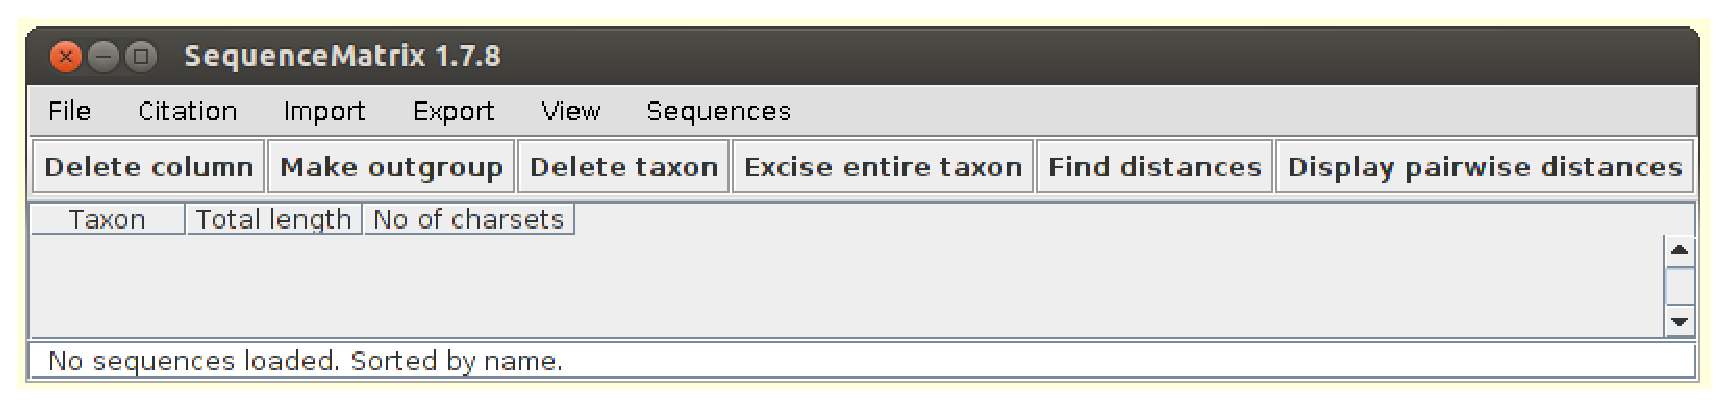
\includegraphics[scale=0.5]{figures/tut7/seqmatrix_1.eps}}
	{\caption[Janela de abertura de SequenceMatrix]{Janela de abertura de SequenceMatrix.}\label{tut7:fig:seqmatrix_1}}
  \end{figure}

%%%%%%%%%%%%%%%%%%%%%%%%%%% FIM DA FIGURA SEQUENCEMATRIX 1 %%%%%%%%%%%%%%%%%%%%%

Para importar partições de dados basta selecionar \texttt{Import/Add sequence} no menu principal. No exemplo abaixo (Figura \ref{tut7:fig:seqmatrix_2}), eu adicionei a primeira partição que estava em um arquivo chamado \texttt{sequencematrix\_1.fas}.


%%%%%%%%%%%%%%%%%%%%%%%%%%% FIGURA SEQUENCEMATRIX 2 %%%%%%%%%%%%%%%%%%%%%%%%%%%
%  \vspace{-1em}
  \begin{figure}[H]
    %\ffigbox[\FBwidth]
       \centering
      {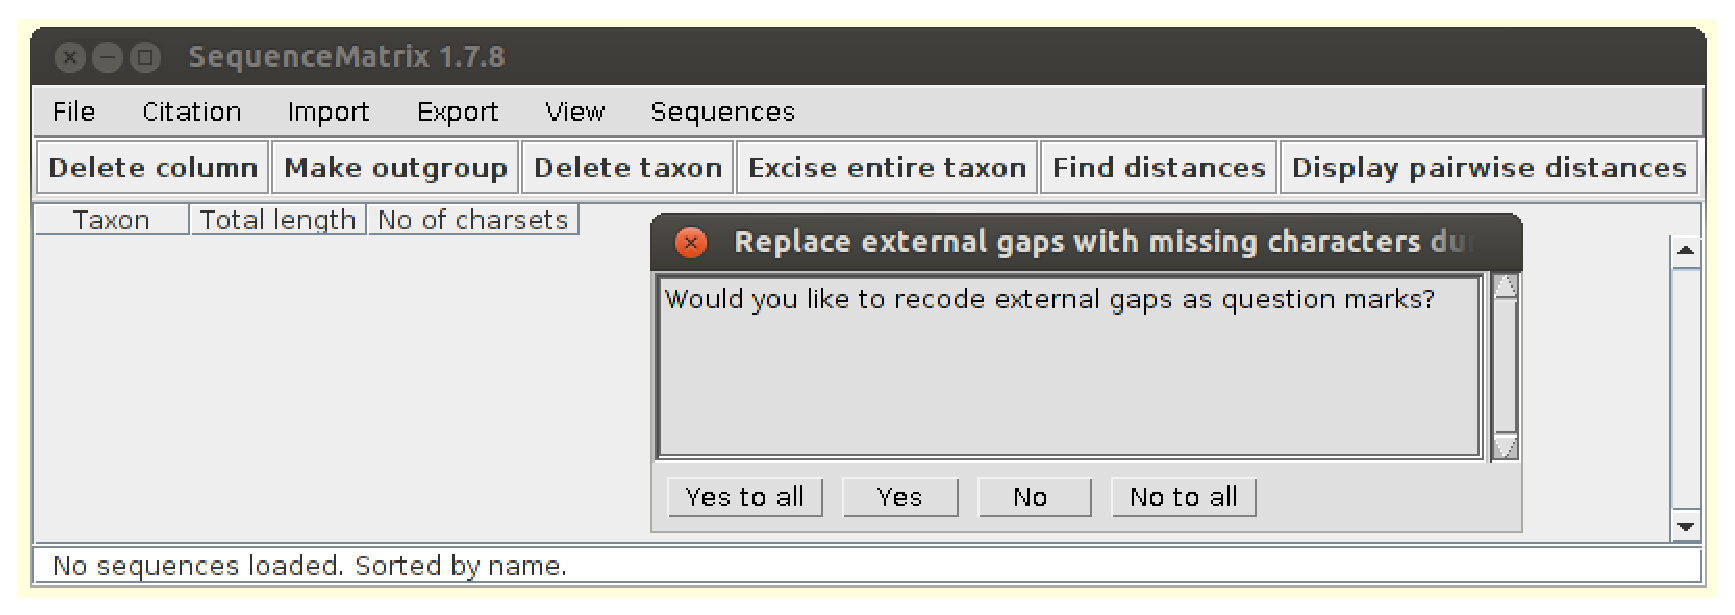
\includegraphics[scale=0.5]{figures/tut7/seqmatrix_2.eps}}
	{\caption[Janela de importanção de SequenceMatrix]{Janela de importação de SequenceMatrix.}\label{tut7:fig:seqmatrix_2}}
  \end{figure}

%%%%%%%%%%%%%%%%%%%%%%%%%%% FIM DA FIGURA SEQUENCEMATRIX 2 %%%%%%%%%%%%%%%%%%%%%

SequenceMatrix irá lhe perguntar se você deseja substituir os \textit{gaps} por \texttt{?}. Você deverá sempre selecionar \textit{No to all}, a não ser que você realmente queira tratar eventos de INDELs como \textit{missing data}. Em breve iremos discutir esse aspecto da análise filogenética da dados moleculares.\\


Em alguns casos, o programa poderá lhe perguntar se você deseja usar o nome do táxon ou da sequência (Figura \ref{tut7:fig:seqmatrix_2b}). Você deverá optar pelo nome da sequência, caso contrário, o programa gerará -- neste caso em particular -- terminais com o mesmo nome. Isso lhe traria proplemas mais adiante. Minha sugestão é que você configure os nomes dos terminais (ou sequências) da forma mais simples e informativa possível nesse estágio de sua análise -- antes de concatená-los. Lembre-se que você poderá substituir esses nomes no final, quando for gerar figuras e ou avaliar resultados. Quanto mais simples os nomes são, mais fácil se torna a tarefa de gerenciar arquivos e evitar erros, principalmente se você está lidando com várias bases de dados para os mesmos terminais


%%%%%%%%%%%%%%%%%%%%%%%%%%% FIGURA SEQUENCEMATRIX 2 %%%%%%%%%%%%%%%%%%%%%%%%%%%
%  \vspace{-1em}
  \begin{figure}[H]
    %\ffigbox[\FBwidth]
       \centering
      {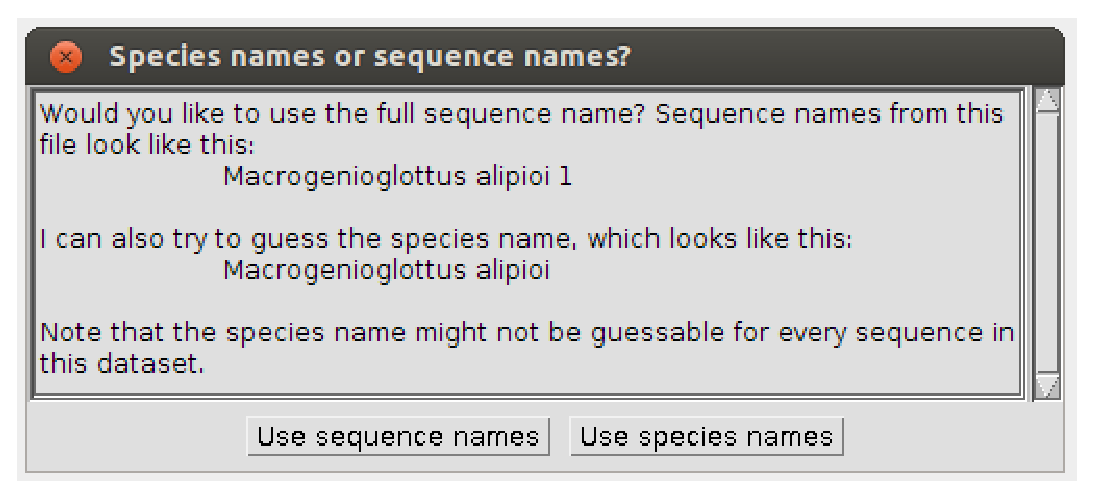
\includegraphics[scale=0.7]{figures/tut7/seqmatrix_2b.eps}}
	{\caption[Janela de seleção de nomes em SequenceMatrix]{Janela de de seleção de nomes em SequenceMatrix.}\label{tut7:fig:seqmatrix_2b}}
  \end{figure}

%%%%%%%%%%%%%%%%%%%%%%%%%%% FIM DA FIGURA SEQUENCEMATRIX 2 %%%%%%%%%%%%%%%%%%%%%

Ao importar as sequências, você deverá obter resultado semelhante ao ilustrado na Figura \ref{tut7:fig:seqmatrix_3}. SequenceMatrix informa alguns detalhes sobre os dados importados, tais como número de terminais, tamanho das sequências e presença de INDELs.\\

%%%%%%%%%%%%%%%%%%%%%%%%%%% FIGURA SEQUENCEMATRIX 3 %%%%%%%%%%%%%%%%%%%%%%%%%%%
%  \vspace{-1em}
  \begin{figure}[H]
    %\ffigbox[\FBwidth]
       \centering
      {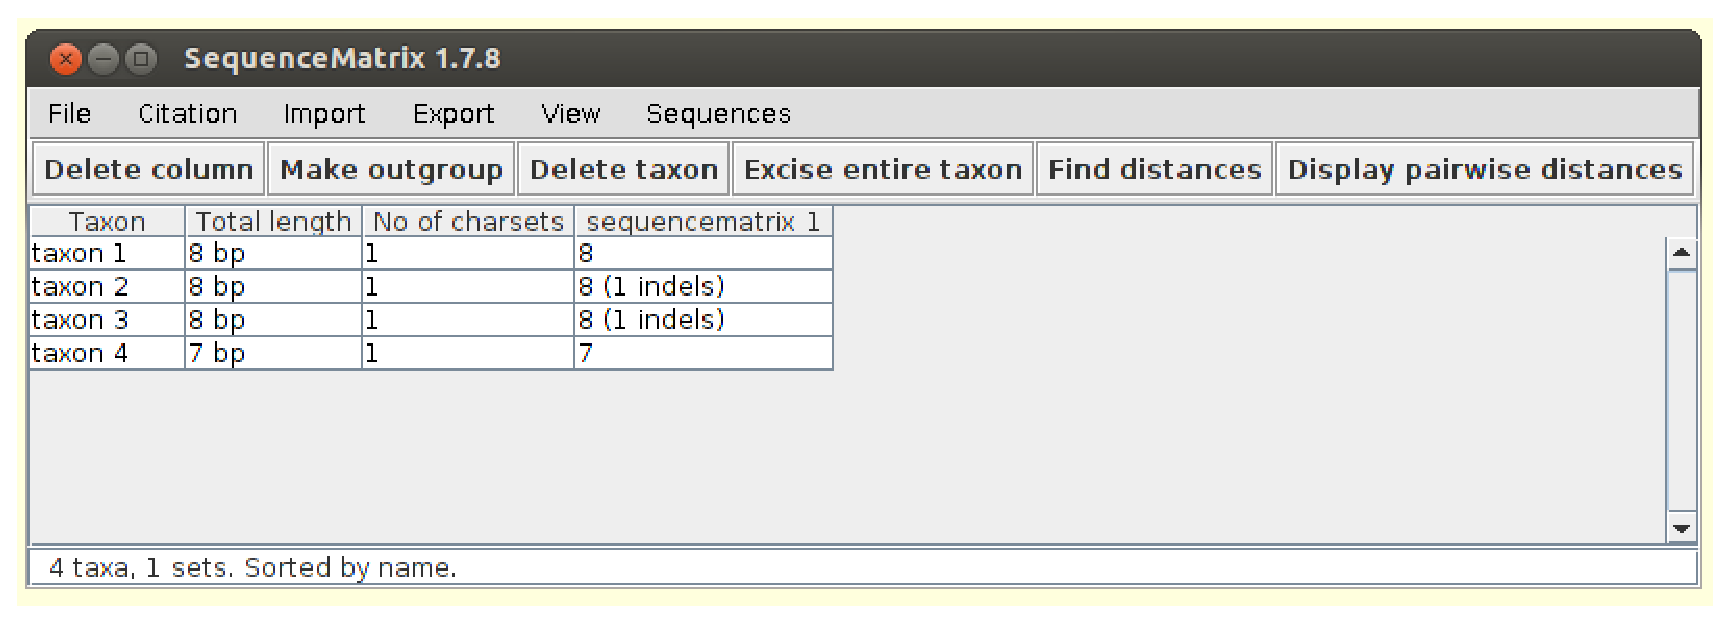
\includegraphics[scale=0.5]{figures/tut7/seqmatrix_3.eps}}
	{\caption[Sequências importadas em SequenceMatrix]{Sequências importadas em SequenceMatrix.}\label{tut7:fig:seqmatrix_3}}
  \end{figure}

%%%%%%%%%%%%%%%%%%%%%%%%%%% FIM DA FIGURA SEQUENCEMATRIX 3 %%%%%%%%%%%%%%%%%%%%%

Para importar todas as partições da Figura \ref{tut7:fig:partitions} basta repetir a tarefa. SequenceMatrix importa matrizes de TNT da mesma forma que importa sequências em formato FASTA. A importação de todas as partições é ilustrada na figura seguinte (Figura \ref{tut7:fig:seqmatrix_4}):

%%%%%%%%%%%%%%%%%%%%%%%%%%% FIGURA SEQUENCEMATRIX 3 %%%%%%%%%%%%%%%%%%%%%%%%%%%
%  \vspace{-1em}
  \begin{figure}[H]
    %\ffigbox[\FBwidth]
       \centering
      {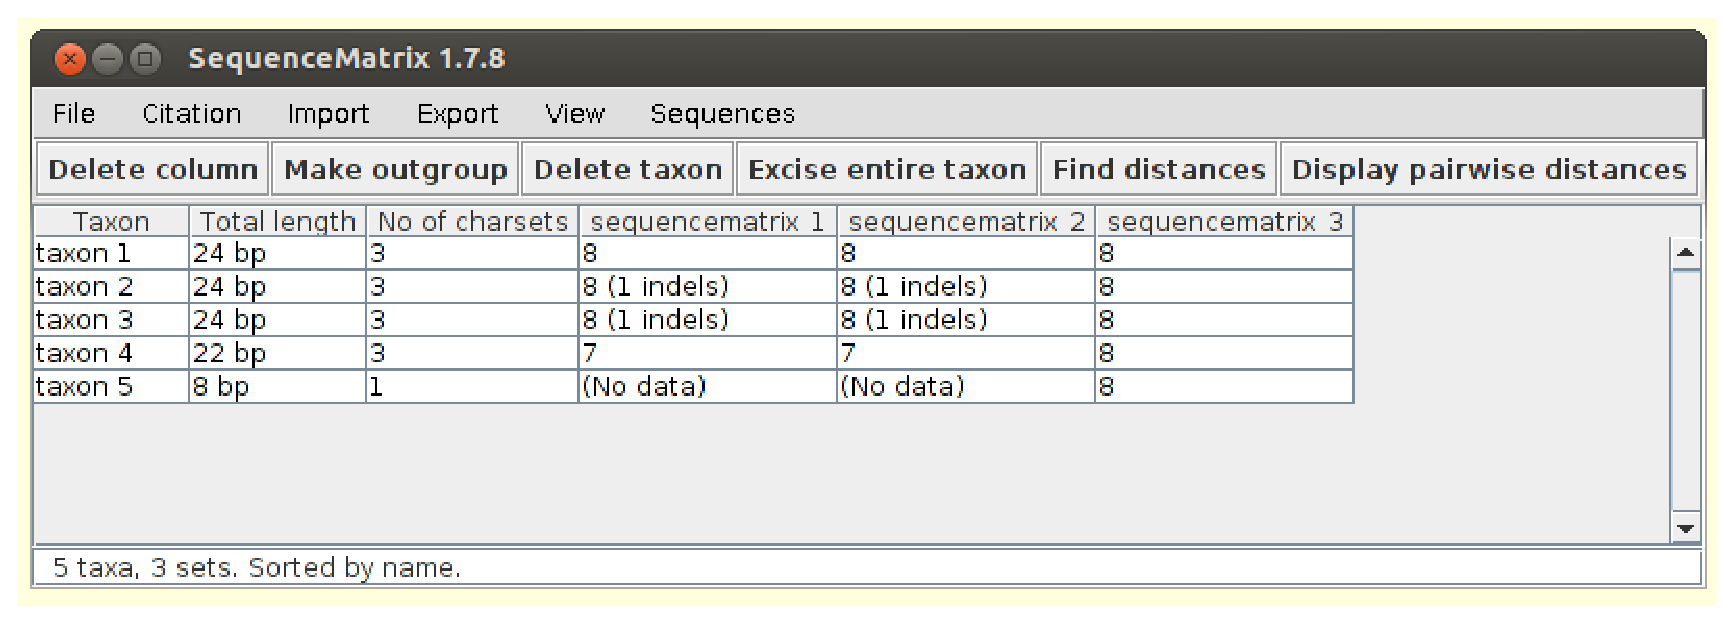
\includegraphics[scale=0.5]{figures/tut7/seqmatrix_4.eps}}
	{\caption[Partições importadas em SequenceMatrix]{Partições importadas em SequenceMatrix.}\label{tut7:fig:seqmatrix_4}}
  \end{figure}

%%%%%%%%%%%%%%%%%%%%%%%%%%% FIM DA FIGURA SEQUENCEMATRIX 3 %%%%%%%%%%%%%%%%%%%%%

Para exportar esses dados, basta selecionar uma das opções disponíveis em \texttt{Export} do menu principal. No exemplo abaixo eu selecionei a opção \texttt{Export/Export sequences as TNT}. O arquivo de exportação terá a seguinte configuração:\\

\scriptsize

\noindent\texttt{nstates~dna;}

\noindent\texttt{xread}

\noindent\texttt{'Exported~by~SequenceMatrix~1.7.8~on~Tue~Apr~22~09:39:44~BRT~2014.'}

\noindent\texttt{24~5}

\noindent\texttt{taxon\_1~AAAACCCCGGGGTTTT00000001}

\noindent\texttt{taxon\_2~AAA-CCCCGGG-TTTT11000000}

\noindent\texttt{taxon\_3~AAAA-CCCGGGG-TTT11110000}

\noindent\texttt{taxon\_4~AAAACCC-GGGGTTT-11111100}

\noindent\texttt{taxon\_5~????????????????11111110;}\\

\noindent\texttt{xgroup}

\noindent\texttt{=0~(sequencematrix\_1)	0~1~2~3~4~5~6~7~}

\noindent\texttt{=1~(sequencematrix\_2)	8~9~10~11~12~13~14~15~}

\noindent\texttt{=2~(sequencematrix\_3)	16~17~18~19~20~21~22~23~}

\noindent\texttt{;}\\

\noindent\texttt{agroup}

\noindent\texttt{=0~(CHARSETS\_ATLEAST\_3)~0~1~2~3}

\noindent\texttt{=1~(CHARSETS\_ATLEAST\_2)~0~1~2~3}

\noindent\texttt{=2~(TAXA\_HAVING\_sequencematrix\_1)~0~1~2~3}

\noindent\texttt{=3~(TAXA\_HAVING\_sequencematrix\_2)~0~1~2~3}

\noindent\texttt{=4~(TAXA\_HAVING\_sequencematrix\_3)~0~1~2~3~4}

\noindent\texttt{;}


\normalsize

No exemplo acima, a matrix de dados contempla todas as partições e insere pontos de interrogação para os caracteres das duas primeira partições nas quais o \texttt{taxon\_5} não está representado. Há dois blocos adicionais neste arquivo. O primeiro deles é o \texttt{xgroup} que define grupos de caracteres. O segundo é o \texttt{agroup} que define grupos de táxons em TNT. Esses blocos são utilizados em TNT para manipular grupos como um todo -- para maiores detalhes veja documentação de TNT.\\


\stepcounter{ex}
\begin{blackBlock}{\textbf{Exercício 7.\arabic{ex}}}\label{tut7:ex:ex4}

Neste exercício você deverá transformar os arquivos que gerou no Exercício 7.3 em arquivos no formato de TNT. As tarefas específicas a serem realizadas são as sequintes:

\end{blackBlock}

\begin {myindentpar}{0.3cm}
\begin{enumerate}[\itshape i.]
	\item{Gerar arquivos no formato TNT para cada partição de \textcite{dias_et_al_2013}.}
	\item{Gerar um arquivo no formato TNT no qual todas as partições estão representadas.}
	\item{Analisar estes arquivos em TNT e fazer um resumo abaixo no qual você compara os resultados que você obteve com a topologia apresentada na Figura 11 (pg. 294) de \textcite{dias_et_al_2013}.}
\end{enumerate}
\end{myindentpar}

\begin{center}
\noindent\line(1,0){400}\\
\line(1,0){400}\\
\line(1,0){400}\\
\line(1,0){400}\\
\line(1,0){400}\\
\line(1,0){400}\\
\line(1,0){400}\\
\line(1,0){400}\\
\line(1,0){400}\\
\line(1,0){400}\\
\end{center}
\newpage
%%%%%%%%%%%%%%%%%%%%%%%%%%%% HERE ENDS TEXT AND ADDS REFERENCES %%%%%%%%%%%%%%%%%%%%%%%%%%%% 
\section{Referências}\label{tut7:refs}
\printbibliography[heading=none]
\end{refsection}
%

